%!TEX root = ../thesis.tex

\chapter{Top Quark Mass Measurement}
\label{c:top_mass_analysis}
\ifpdf
    \graphicspath{{05_Mass_analysis/plots/}}
\else
    \graphicspath{{05_Mass_analysis/plots/EPS/}{05_Mass_analysis/plots/}}
\fi

The top quark mass measurement using 2011 LHC data recorded by the CMS detector at a centre of mass energy of $\sqrt s
=$ \SI{7}{\TeV} is presented in this chapter. The analysis was a cross-check to the official CMS top quark mass
measurement at \SI{7}{\TeV} in the lepton plus jets channel published in 2012 \autocite{top_mass_ljets_CMS}, which
currently remains the most precise single measurement of the top quark mass. Only the electron plus jets channel is
described in this thesis, as the muon side of the analysis was performed by a different group at CERN, although in close
collaboration.

The mass extraction technique used in this analysis, referred to as the ideogram method, is essentially the same as one
used in the CMS measurement of the mass difference between top and antitop quarks \autocite{mass_difference_CMS} and the
top quark mass measurement in 2010 \autocite{top_mass_ljets_CMS_2010}. In this chapter, this technique is described in
detail. Additionally, data and Monte Carlo samples, event selection process, the kinematic fit used for \ttbar
reconstruction, as well as the calibration of the ideogram method, systematic uncertainties and the final result are
presented in relevant sections of the chapter.

\section{Data and Simulation}
\label{s_top_mass:data_and_simulation}

\subsection{Data}
\label{ss_top_mass:data}
The data used in this work is the full 2011 dataset recorded by the CMS detector with a total integrated luminosity of
\SI{5.0 \pm 0.1}{\fbinv}. As only the electron channel is covered by this particular analysis, all data were
pre-selected by single electron plus jets high level triggers, described in detail in Chapter \ref{c:service_work}.

% \begin{itemize}
%   \item electron + 3 (PF)jets
%   \item isolated electron + 3 (PF)jets
% \end{itemize}

% \begin{itemize}
% 	\item /ElectronHad/Run2011A-May10ReReco-v1/AOD
% 	\item /ElectronHad/Run2011A-PromptReco-v4/AOD
% 	\item /ElectronHad/Run2011A-05Aug2011-v1/AOD
% 	\item /ElectronHad/Run2011A-PromptReco-v6/AOD
% 	\item /ElectronHad/Run2011B-PromptReco-v1/AOD
% \end{itemize}

\subsection{Simulation of signal and background processes}
\label{ss_top_mass:signal_and_background}

To develop and test any analysis technique in particle physics, simulated events from Monte Carlo (MC) generators as
well as a working simulation model of the detector are inevitably needed. In this analysis, \ttbar signal decays and
background processes were generated with a set of different MC generators including \MADGRAPH \autocite{MadGraph},
\PYTHIA \autocite{Pythia,Pythia6.4} and \POWHEG \autocite{POWHEG}. A supplementary package (\TAUOLA \autocite{TAUOLA})
was used for the tau lepton decay description. In this section, all the event generators as well as the different MC
tunes used for evaluation of systematic uncertainties are briefly described. Additionally, the \GEANTfour-based
\autocite{GEANT4} CMS detector simulation is mentioned, and finally Monte Carlo samples for all processes are
presented.

\subsubsection{Monte Carlo event generators}
\label{sss_top_mass:MC_generators}

Simulation of \ttbar signal and background processes, described in Section~\ref{s:top_quak_physics}, was performed using
several Monte Carlo event generators. The process of simulating a hadron collision event is rather complicated, and
usually includes generation of the following steps:

\begin{enumerate}[label=\textbullet]
	\item incoming hadrons (protons);
	\item hard scattering of partons;
	\item boson radiation (\Z, \photon, \cPg);
	\item parton shower;
	\item hadronisation of partons.
\end{enumerate}

The performance of MC generators is usually optimised for one or more of these steps, therefore they two or more
generators often used in combination, e.g.\ \ttbar signal is modelled with \MADGRAPH and \PYTHIA. Standalone generators
can also be used for modelling theory systematic effects, which is also exploited in this thesis.
%(\MCATNLO, \POWHEG + \PYTHIA).

\begin{description}[wide=\parindent, style=standard, labelsep=0pt]
\item [\MADGRAPH] \autocite{MadGraph} is a matrix-element Monte Carlo event generator. For any renormalisable
Lagrangian-based model it produces all possible Feynman diagrams and automatically generates its matrix elements at the
tree level, performing the integration over all phase-space. This calculation is then used to produce the \xsect of
various processes and subprocesses as well as partons and kinematics of an event, including decays that are described
using spin correlations. Partons from matrix element calculations are then matched to parton showers from hadronisation
of quarks and gluons, which is simulated in \PYTHIA (see below) along with the fragmentation of initial protons and the
soft scattering of underlying event (mentioned in Section~\ref{sss:JEC}). The matching is done according to the
so-called MLM prescription \autocite{MLM} if a parton-jet pair satisfies a certain $\Delta R$ separation criterion. If
no or more than one matched jets are found, events are rejected. There is also a certain transverse energy threshold
requirement for the partons to be considered in the matching. Default values as well as variations used to estimate the
systematic effect of the matching threshold are shown in Table~\ref{tab:systematic_mc_variations}.

\item [\PYTHIA] \autocite{Pythia,Pythia6.4} is one of the most widely used MC generators in high energy physics. It is a
standard tool used for simulation of quark and gluon hadronisation, multi-particle production, beam remnants, initial
protons fragmentation, etc. In this work, \PYTHIA is used to generate QCD multi-jet production, and to simulate the
underlying event on top of other generators providing partons from hard processes.

\item [\MCATNLO] \autocite{MCatNLO} is a parton shower MC generator providing next-to-leading order (NLO) corrections
for a simulated process. It represents a major improvement in precision and accuracy of physics simulations comparing to
leading order (LO) generators like \PYTHIA. NLO implementation can handle additional partons in the final state coming
from the hard scattering, which is not possible with LO calculations. Therefore it includes additional dynamic features,
giving a major advantage for heavy flavour physics.

\item [\POWHEG] (Positive Weight Hardest Emission Generator) \autocite{POWHEG} also works at NLO precision. Its main
difference to \MCATNLO generator lies in the order of process generation: \POWHEG initially generates the hardest
radiation. This technique allows to avoid double-counting coming from subsequent radiation which may happen with
\MCATNLO method when matching QCD NLO calculations with parton showers.
%http://theory.fnal.gov/seminars/slides/2008/COleari.pdf

\end{description}

\subsubsection{Matching Threshold and Factorisation Scale}
\label{sss_top_mass:matching_and_factorisation}
%https://twiki.cern.ch/twiki/bin/view/CMS/MadGraphStandardModel

As described above with the example of \MADGRAPH generator, there is a certain threshold for partons transverse momenta
from matrix element calculations to be matched with parton showers, often referred to as ME-PS threshold. To estimate
the systematic uncertainty arising from it, additional MC samples were generated with the value of the threshold either
halved or doubled. This procedure was performed for signal \ttjets and background \WpJets and \ZpJets samples.
Similarly, the systematic effect of the choice of factorisation scale $Q^2$ (described in
Section~\ref{ss:top_production}) is determined. A summary of central values and variations used to estimate these
systematic uncertainties is shown in Table~\ref{tab:systematic_mc_variations}, whereas the list of systematic MC samples
is shown in Table~\ref{tab:top_mass_systematic_samples}.

\begin{table}[!htbp] \centering
\begin{tabular}{|l|r|r|}
\toprule
parameter & factorisation scale & matching threshold \\ 
\midrule
\multicolumn{3}{|c|}{\ttbar events} \\
\midrule
central value & $Q^2 = \mtop^2 + \sum\limits_{\rm jets} \pt^2$ & \SI{20}{\GeV} \\[2.5ex]
variations  &$\left(0.5 \cdot Q\right)^2, \left(2 \cdot Q\right)^2$ &\SIlist{10;40}{\GeV}\\
\midrule
\multicolumn{3}{|c|}{\WpJets and \ZpJets events} \\
\midrule
central value & $Q^2 = m_{\W/\Z}^2 + \sum\limits_{\rm jets} \pt^2$ & \SI{10}{\GeV} \\[2.5ex]
variations &$\left(0.5 \cdot Q\right)^2, \left(2 \cdot Q\right)^2$&\SIlist{5;20}{\GeV}\\
\bottomrule
\end{tabular}
\caption{Central values and variations used for systematic uncertainties of
 factorisation/renormalisation scale ($Q^2$) and matrix element -- parton shower
 (ME-PS) matching in \MADGRAPH MC generator.}
\label{tab:systematic_mc_variations} 
%https://twiki.cern.ch/twiki/bin/view/CMS/MadGraphStandardModel
\end{table}

\subsubsection{CMS detector simulation}
\label{sss_top_mass:detector_simulation}

Detector simulation is an essential final step on top of the full physics simulation of proton-proton collisions. All
generated particles resulting from these collisions are propagated to the simulated layers of the detector so that their
interaction with the detector material and detector response can also be modelled. The CMS simulation is based on the
\GEANTfour (GEometry ANd Tracking \autocite{GEANT4}) package, which is implemented in CMS software \CMSSW
\autocite{CMSSW}. This package fully recreates the geometry of the detector, including all its subsystems as well as a
detailed map of the magnetic field.

In general, the simulation procedure includes modelling of the following steps:
\begin{enumerate}[label=\textbullet]
	\item interaction region;
	\item particles traversing all the layers of the detector and the interaction processes;
	\item multiple interactions per beam crossing (pile-up) and event overlay effects;
	\item digital readout of the detector (digitisation).
\end{enumerate}
%https://twiki.cern.ch/twiki/bin/view/CMSPublic/SWGuideSimulation

The data stream generated with this process is very similar to the output of the real detector, although naturally in
addition to reconstructed objects, generated events also include collections of generated objects, allowing users to
access the Monte Carlo truth information, which is essential for any particle physics analysis.

\subsubsection{Monte Carlo samples}
\label{sss_top_mass:mc_samples}

The nominal signal \ttbar MC sample used in this analysis was generated using the \MADGRAPH generator with a top quark
mass of \mtop = \SI{172.5}{\GeV}. To calibrate the mass extraction technique, as explained in
Section~\ref{s_top_mass:calibration}, 8 additional \ttbar samples were used with different top quark masses ranging
between \SIlist{161.5;184.5}{\GeV}. The \WpJets and \ZpJets background processes (see Section~\ref{ss:backgrounds}) were
also generated with \MADGRAPH, whereas the single top background was generated with \POWHEG generator. A full list of
signal \ttbar and background MC samples with values of cross section, numbers of generated events and corresponding
integrated luminosities is shown in Table~\ref{tab:top_mass_mc_samples}. All samples were produced using the CTEQ6L
Parton Distribution Functions (PDF) \autocite{CTEQ}.

The QCD background samples are available in two different sets, one of which is pre-filtered to contain jets with high
electromagnetic content ($e/\gamma$ enriched), and the second one is enriched with electrons coming from decays of heavy
flavour quarks ($\cPqb/\cPqc \rightarrow \cPq e\nu$). This pre-selection is performed at generator level, to ensure
reasonable statistics after the \ttbar selection imposed in top quark analyses with electrons in the final state. Both
sets of QCD samples are generated with \PYTHIA generator in different exclusive bins of \pthat (i.e.\ transverse
momentum of the outgoing partons defined in the rest frame of the hard process). The $\gamma$+jets MC samples were
produced with \MADGRAPH in different bins of \HT at generator level, which denotes the sum of transverse momenta of all
high-\pt objects. Table~\ref{tab:top_mass_background_qcd} gives a list of QCD and $\gamma$+jets samples with values of
production cross sections, pre-selection efficiencies, numbers of generated events and corresponding integrated
luminosities.

%http://cms.pd.infn.it/software/meetings/MultiMuon/doc/pthat-firstlook-v3.pdf
%gamma plus jets samples were not even used?

Finally, Table~\ref{tab:top_mass_systematic_samples} lists the additional samples generated to allow estimation of the
systematic uncertainties due to factorisation scale and matching threshold choices, as discussed earlier.

%in Section~\ref{sss_top_mass:matching_and_factorisation}.


\begin{table}[!htbp]
\centering
\caption{Signal and background Monte Carlo samples with cross sections at $\sqrt s = \SI{7}{\TeV}$, numbers of generated
events and corresponding integrated luminosities.}
\label{tab:top_mass_mc_samples}
\begin{tabular}{|l|l|r|r|r|}
\toprule
Process & Generator & $\sigma$ (\pb) & \# events & $\int\lumi dt$ (\fbinv)\\
\midrule
\ttjets & \MADGRAPH & & & \\
\hspace{5 mm}\mtop = \SI{161.5}{\GeV} & & 157.5 & 1620072 & 10.3\\
\hspace{5 mm}\mtop = \SI{163.5}{\GeV} & & 157.5 & 1633197 & 10.4\\
\hspace{5 mm}\mtop = \SI{166.5}{\GeV} & & 157.5 & 1669034 & 10.6\\
\hspace{5 mm}\mtop = \SI{169.5}{\GeV} & & 157.5 & 1606570 & 10.2\\
\hspace{5 mm}\mtop = \SI{172.5}{\GeV} & & 157.5 & 7490162 & 47.6\\
\hspace{5 mm}\mtop = \SI{175.5}{\GeV} & & 157.5 & 1538301 & 9.8\\
\hspace{5 mm}\mtop = \SI{178.5}{\GeV} & & 157.5 & 1648519 & 10.5\\
\hspace{5 mm}\mtop = \SI{181.5}{\GeV} & & 157.5 & 1665350 & 10.6\\
\hspace{5 mm}\mtop = \SI{184.5}{\GeV} & & 157.5 & 1671859 & 10.6\\
\midrule
\WpJets ($\W \rightarrow l\nu$) & \MADGRAPH & 31314 & 81345381 & 2.6 \\
% \hspace{5 mm}\W + 1 jet & & 4480 & 76051609 & 17.0 \\
% \hspace{5 mm}\W + 2 jet & & 1674 & 25400546 & 15.2 \\
% \hspace{5 mm}\W + 3 jet & & 484.7 & 7541595 & 15.6 \\
% \hspace{5 mm}\W + 4 jet & & 211.7 & 13133738 & 62.0 \\
\midrule
$\Z/\gamma^* \rightarrow l^+l^- $ + jets, $m(ll) > \SI{50}{\GeV}$ & \MADGRAPH & 3048 & 36222153 & 11.9 \\
\midrule
Single top & \POWHEG & & & \\
\hspace{5 mm} top $t$-channel & & 42.6 & 3814228 & 89.5 \\
\hspace{5 mm} anti-top $t$-channel & & 22.0 & 1944822 & 88.4 \\
\hspace{5 mm} top $s$-channel & & 2.72 & 259971 & 92.6 \\
\hspace{5 mm} anti-top $s$-channel & & 1.49 & 137980 & 92.6 \\
\hspace{5 mm} top $tW$-channel & & 5.3 & 814390 & 153.7 \\
\hspace{5 mm} anti-top $tW$-channel & & 5.3 & 809984 & 152.8 \\
\bottomrule
\end{tabular}
\end{table}

% \begin{table}[!hbth] \centering
% \begin{tabular}{lrrr}
% \toprule
% process & $\sigma$ (\pb) & \# events & $\int\lumi dt$ \fbinv\\
% \midrule
% \WpJets ($\W \rightarrow l\nu$) & 31314 & 81345381 & 2.6 \\
% \W + 1 jet ($\W \rightarrow l\nu$) & 4480 & 76051609 & 17.0 \\
% \W + 2 jet ($\W \rightarrow l\nu$) & 1674 & 25400546& 15.2 \\
% \W + 3 jet ($\W \rightarrow l\nu$) & 484.7 & 7541595 & 15.6 \\
% \W + 4 jet ($\W \rightarrow l\nu$) & 211.7 & 13133738 & 62.0 \\
% $\Z/\gamma^* \rightarrow l^+l^-, m(ll) > \SI{50}{\GeV}$ + jets & 3048 & 36222153 & 11.9 \\
% Single top t-channel & 42.6 & 3814228 & 89.5 \\
% Single anti-top t-channel & 22.0 & 1944822 & 88.4 \\
% Single top s-channel & 2.72 & 259971 & 92.6 \\
% Single anti-top s-channel & 1.49 & 137980 & 92.6 \\
% Single top tW-channel & 5.3 & 814390 & 153.7 \\
% Single anti-top tW-channel & 5.3 & 809984 & 152.8 \\
% \bottomrule
% \end{tabular}
% \caption{Background Monte Carlo samples, their cross sections at a \CoM energy
% of \SI{7}{\TeV}, numbers of generated events and corresponding integrated
% luminosities.}
% \label{tab:top_mass_background_mc}
% \end{table}

\begin{table}[!htbp] 
\centering
\caption{QCD multi-jet background and $\gamma$ + jets MC samples with cross sections at $\sqrt s =
\SI{7}{\TeV}$, numbers of generated events and corresponding integrated luminosities.
% EM-enriched samples are preselected to include jets with higher electromagnetic content;
% $\cPqb/\cPqc \rightarrow e\nu$ samples are preselected to include leptonic ($e\nu$) in-flight decays of b- and c-quarks.
}
\label{tab:top_mass_background_qcd}
\resizebox{\textwidth}{!}{
\begin{tabular}{|l|l|r|r|r|r|}
\toprule
Process & Generator & $\sigma$ (\pb) & filter efficiency & \# events & $\int\lumi dt$ (\fbinv)\\
\midrule
QCD ($e/\gamma$ enriched)  & \PYTHIA & & & & \\
\hspace{5 mm}\SIrange[range-phrase = $~<\pthat<~$]{20}{30}{\GeV} & & \num{2.355d8} & \num{7.3d-3} & 34720808 & \num{2.0d-2} \\
\hspace{5 mm}\SIrange[range-phrase = $~<\pthat<~$]{30}{80}{\GeV}  & & \num{5.93d7}& \num{0.059} &  70375915 & \num{2.0d-2} \\
\hspace{5 mm}\SIrange[range-phrase = $~<\pthat<~$]{80}{170}{\GeV} & & \num{9.06d5} & \num{0.148} &  8150669& \num{6.1d-2} \\
\midrule
QCD ($\cPqb/\cPqc \rightarrow e\nu$) & \PYTHIA & & & & \\
\hspace{5 mm}\SIrange[range-phrase = $~<\pthat<~$]{20}{30}{\GeV} & & \num{2.355d8} & \num{4.6d-4} & 2002588 & \num{1.8d-2} \\
\hspace{5 mm}\SIrange[range-phrase = $~<\pthat<~$]{30}{80}{\GeV} & & \num{5.93d7}& \num{2.34d-3} & 2030030 & \num{1.5d-2} \\
\hspace{5 mm}\SIrange[range-phrase = $~<\pthat<~$]{80}{170}{\GeV} & & \num{9.06d5} & \num{0.0104} & 1082690 & \num{0.1} \\
\midrule
$\gamma$ + jets & \MADGRAPH & & & & \\
\hspace{5 mm}\SIrange[range-phrase = $~<\HT<~$]{40}{100}{\GeV} & & \num{23620} & 1 & 12730863 & \num{0.5} \\
\hspace{5 mm}\SIrange[range-phrase = $~<\HT<~$]{100}{200}{\GeV} & & \num{3476} & 1 & 1536287 & \num{0.4} \\
\hspace{5 mm}$\HT >$ \SI{200}{\GeV} & & \num{485} & 1 & 9377168 & \num{19.3} \\
\bottomrule
\end{tabular}
}
\end{table}

\begin{table}[!htbp]
\centering
\caption{Systematic MC samples with cross sections at $\sqrt s = \SI{7}{\TeV}$, numbers of generated events and
corresponding integrated luminosities. Factorisation scale $Q$ and matching threshold systematic uncertainties (see
Section \ref{ss:matching_and_factorisation}) are estimated with variations of \ttjets, \WpJets and \ZpJets samples.}
\label{tab:top_mass_systematic_samples}
\begin{tabular}{|l|l|r|r|r|}
\toprule
Process & Generator & $\sigma$ (\pb) & \# events & $\int\lumi dt$ (\fbinv)\\
\midrule
\ttjets & \MADGRAPH & & & \\
\hspace{5 mm}$0.5~\times$ matching threshold & & 157.5 & 1607808& 10.2 \\
\hspace{5 mm}$2~\times$ matching threshold  & & 157.5 & 4029823& 25.5 \\
\hspace{5 mm}$0.5\times Q$  & & 157.5 & 4004587 & 25.4 \\
\hspace{5 mm}$2\times Q$ & & 157.5 & 3696269 & 23.4 \\
\midrule
\WpJets ($\W \rightarrow l\nu$) & \MADGRAPH & & & \\
\hspace{5 mm}$0.5~\times$ matching threshold & & 29690 & 9956679 & 0.3 \\
\hspace{5 mm}$2~\times$ matching threshold & & 30290 & 10461655 & 0.3 \\
\hspace{5 mm}$0.5 \times Q$ & & 33300 &10092532 & 0.3 \\
\hspace{5 mm}$2 \times Q$ & & 32000 &9784907 &0.3 \\
\midrule
\ZpJets ($\Z \rightarrow ll$) & \MADGRAPH & & & \\
\hspace{5 mm}$0.5~\times$ matching threshold & & 2888 & 1614808& 0.6 \\
\hspace{5 mm}$2~\times$ matching threshold & & 2915 & 1641121 & 0.6 \\
\hspace{5 mm}$0.5 \times Q$ & & 3312 & 1658855 & 0.5 \\
\hspace{5 mm}$2 \times Q$ & & 2954 & 1592742 & 0.5 \\
\bottomrule
\end{tabular}
\end{table}

\clearpage

% \subsection{Pile-up reweighting}
% \label{ss_top_mass:pileup_reweithing}
% Since the number of pile-up vertices in data can be only known after the data-taking, the simulated number of pile-up
% interactions in Monte Carlo may not correspond to the one observed in data. To account for this disagreement between
% data and Monte Carlo, pile-up reweighting procedure is applied to simulated events. don't have the plots for

% electrons. here are some for muons:
% https://indico.cern.ch/getFile.py/access?contribId=1&resId=0&materialId=slides&confId=168447

% \subsection{b-tagging corrections}
% \label{ss_top_mass:btagging_corrections}

\section{Event Selection}
\label{s_top_mass:event_selection}

The event selection applied in this analysis essentially follows the so-called reference selection, i.e.\ the one
recommended by the CMS Top Quark Physics Analysis Group for SM top quark measurements. It is designed to select the
semileptonic signature of a \ttbar decay with an isolated lepton, four jets (including two jets from \cPqb-quarks) and
a neutrino in the form of missing transverse energy. All objects are reconstructed using the particle flow method as
described in Section~\ref{s:object_reconstruction}.

% and use the pile-up subtraction techniques for charged particles (no neutral particle correction) as described in
% Section %\ref{ss:pileup_subtraction}.

As this analysis focuses on the electron channel, the event selection proceeds as follows:

\begin{enumerate}[topsep=\parskip, parsep=\parskip, itemsep=\parskip, leftmargin=\leftmargin]
	\item preselection;
	\item trigger;
	\item electron candidate selection;
	\item dilepton veto;
	\item conversion veto;
	\item muon veto;
	\item jet selection;
	\item b-tagging.
\end{enumerate}

\subsubsection*{Preselection}
Preselection is performed in order to reduce the number of events stored for local analysis. All events are required to
have at least one electron with \ET above \SI{30}{\GeV} within pseudorapidity region of $\abs \eta < 2.5$, or at least
one muon with \pt above \SI{20}{\GeV} and $\abs \eta < 2.1$. Additional event cleaning is performed at this stage to
decrease the number of events with substantial detector noise. A small fraction of events with anomalous HCAL noise is
removed by an HCAL noise filter. Furthermore, beam scraping is mitigated by the appropriate filter requiring at least
\SI{25}{\percent} tracks with high purity if there are more than \num{10} tracks in the event. Finally, the preselection
stage includes the requirement of at least one good primary vertex in the event which has to be located within
\SI{24}{\cm} in the $z$-direction from the centre of CMS and within a radial distance of \SI{2}{\cm}. The primary vertex
is also required to have at least four degrees of freedom which is determined from the vertex fit and is strongly
correlated with the number of tracks compatible with the primary interaction region \autocite{Tacking_PV_results_7TeV}.

%https://twiki.cern.ch/twiki/bin/view/CMS/TWikiTop2011DataMCTrig

\subsubsection*{Trigger}
The trigger requirement is imposed as described in Chapter~\ref{c:service_work}. Essentially, all the events are
required to fire the electron-plus-three-jets trigger in the version current at the time of data-taking. A full list of
triggers can be found in Appendix \ref{a:full_trigger_list}.

\subsubsection*{Electron candidate selection}
Exactly one electron candidate satisfying all the following criteria is required to be present in the event. As the
electron plus jets trigger has a lepton \pt threshold of \SI{25}{\GeV}, the electron candidate transverse momentum is
required to be above \SI{30}{\GeV}, in order to be in the trigger efficiency plateau region. Furthermore, the electron
has to be within the tracker region of $|\eta| < 2.5$ excluding the ECAL barrel-endcap transition regions of $1.4442 <
|\eta| < 1.566$. The CiC electron ID (see Section~\ref{ss:electron_reconstruction}) with the tightest working point
(``HyperTight'') is used for electron identification purposes. This working point provides a misidentification rate of
less than \SI{1}{\pc}, and overall identification efficiency of \SI{75}{\pc} \autocite{CiC_ID}.

In order to only select electrons originating at the interaction vertex, the $x$-$y$ distance ($d_{xy}$) between the
electron track and the interaction point (2D impact parameter) is required to be less than \SI{0.02}{\cm}. The
contribution of electrons inside jets from QCD background events, as well as fake electrons, is reduced by imposing the
PF-based relative isolation cut on the variable \reliso defined in Section~\ref{sss:electron_isolation}. A $\Delta
R$-cone with size of \num{0.3} is used in calculation of the \reliso variable, and events with \reliso $< 0.1$ are
accepted.

\subsubsection*{Dilepton veto}
A veto requirement on a second electron candidate (or dilepton veto) is used to reject events with any additional
electrons. Looser criteria are used to identify the second electron in an event. Namely, the event is rejected if there
is a second electron satisfying a lower \ET threshold of \SI{20}{\GeV} and a looser cut on \reliso ($<0.2$).

Additionally, in order to reduce \ZpJets background, the following veto is applied. If the event contains a second
electron with $\ET > \SI{30}{\GeV}$ and $\reliso < 1.0$ that forms such an invariant mass with the signal electron
candidate that it is close to the \Z mass peak, it is also rejected. The invariant mass window around the \Z peak is
chosen to be $\SI{76}{\GeV} < m_{ee} < \SI{106}{\GeV}$.

%^^not sure if it's actually in reference selection! but looks like I applied it...

\subsubsection*{Conversion veto}
As mentioned in Section~\ref{sss:photon_conversions}, two methods are used in this analysis to remove electrons coming
from photon conversions: missing pixel layers method and partner track matching method. If missing pixel layer hits or a
matching partner track are present in the event, it is rejected.

\subsubsection*{Muon veto}
Other \ttbar channels, including muon and dilepton decay modes, can contaminate events passing the electron plus jets
selection. To reduce this contamination, events containing an isolated global muon (see Section
\ref{ss:muon_reconstruction}) are rejected. The muon is required to have a \pt above \SI{10}{\GeV}, $|\eta| < 2.5$ and
$\reliso < 0.2$ with a $\Delta R$ cone of \num{0.4}.

\subsubsection*{Jet selection and b-tagging}
Final steps in the selection help to further reduce the background by imposing constraints on the number of jets. This
is particularly effective to mitigate the \WpJets contamination, as the number of \WpJets events decreases exponentially
with increasing number of jets. In this analysis, at least four jets with $\pt > \SI{30}{\GeV}$ and $|\eta| < 2.4$ are
required to be present in the event. These jets have to pass the loose PF jet ID (see Section
\ref{ss:jet_reconstruction}). Finally, the CSV b-tagging algorithm with medium working point (Section
\ref{sss:b-tagging}) is used to identify the two \cPqb-quarks from the \ttbar decay.

\begin{figure}[!htp]
   \centering
   \subfloat[]{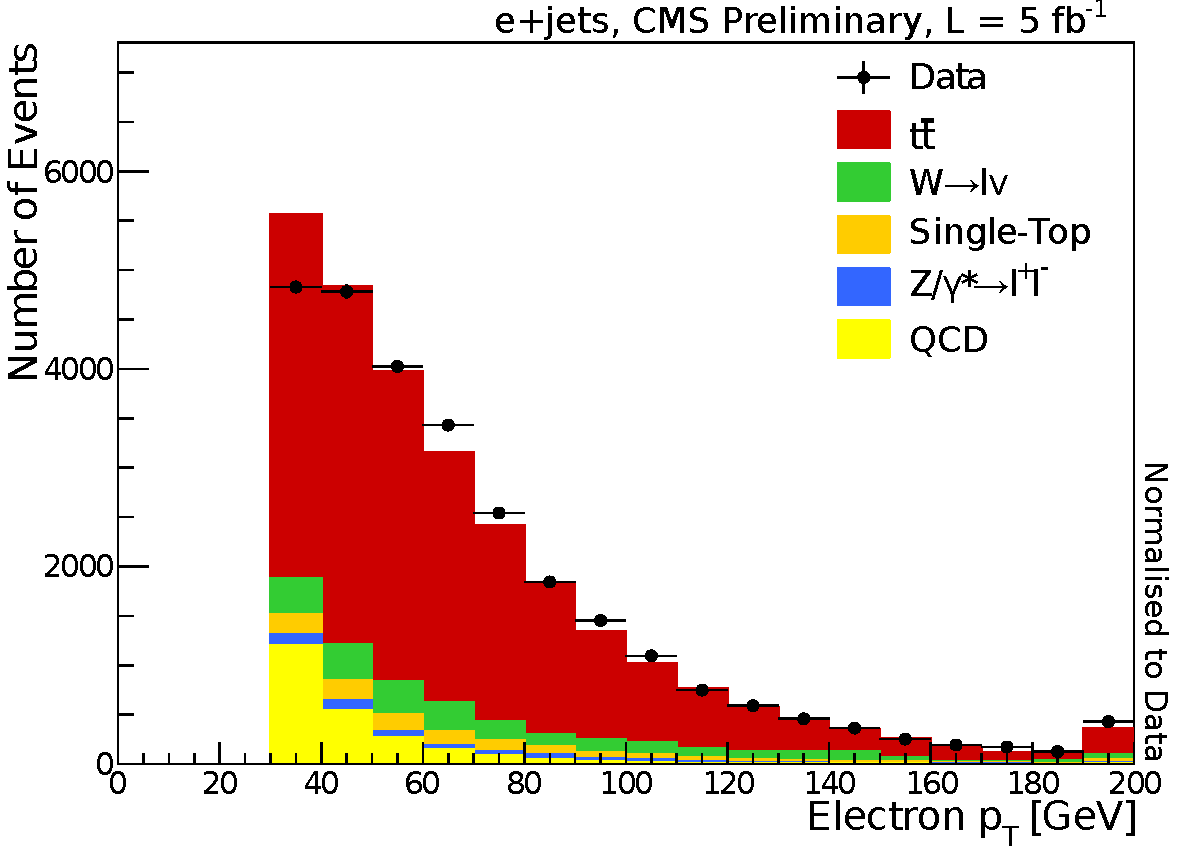
\includegraphics[width=0.5\textwidth]{cmg_electron_pt}}
   \subfloat[]{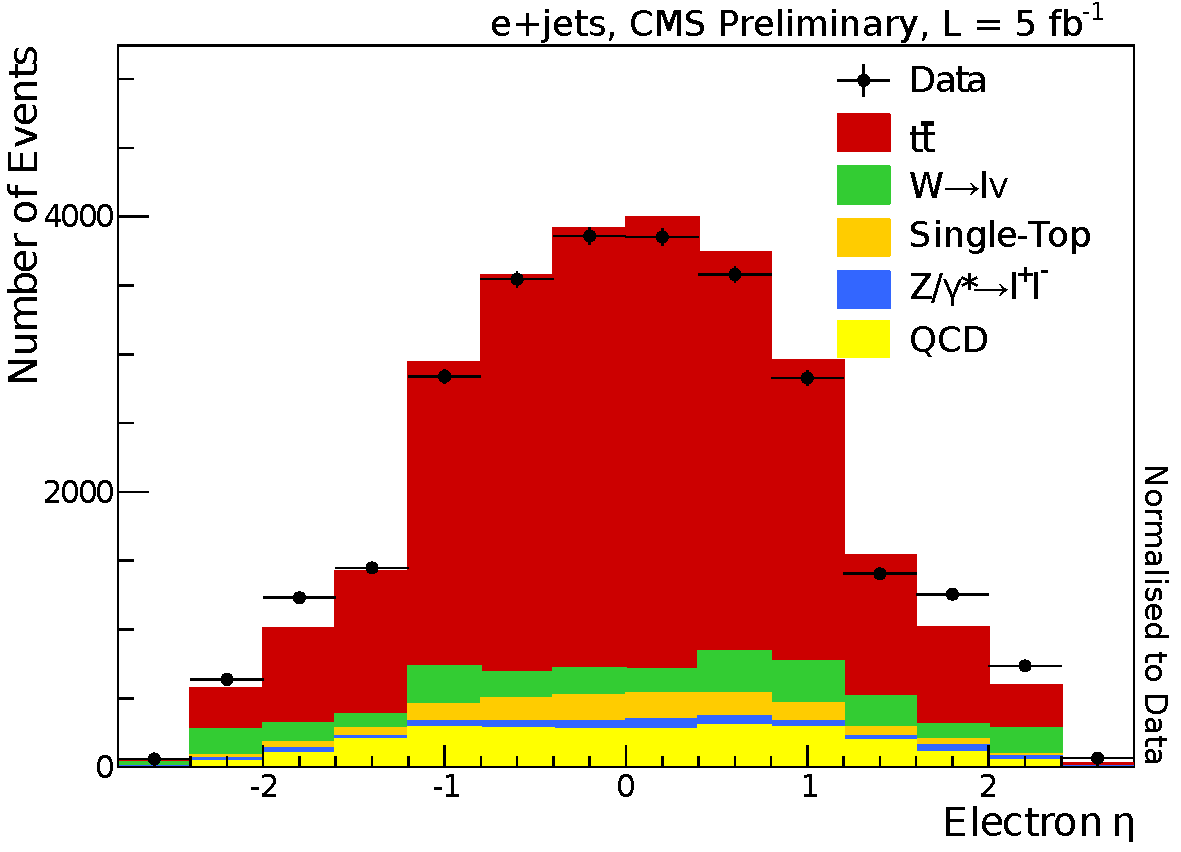
\includegraphics[width=0.5\textwidth]{cmg_electron_eta}}
   \hfill
   \subfloat[]{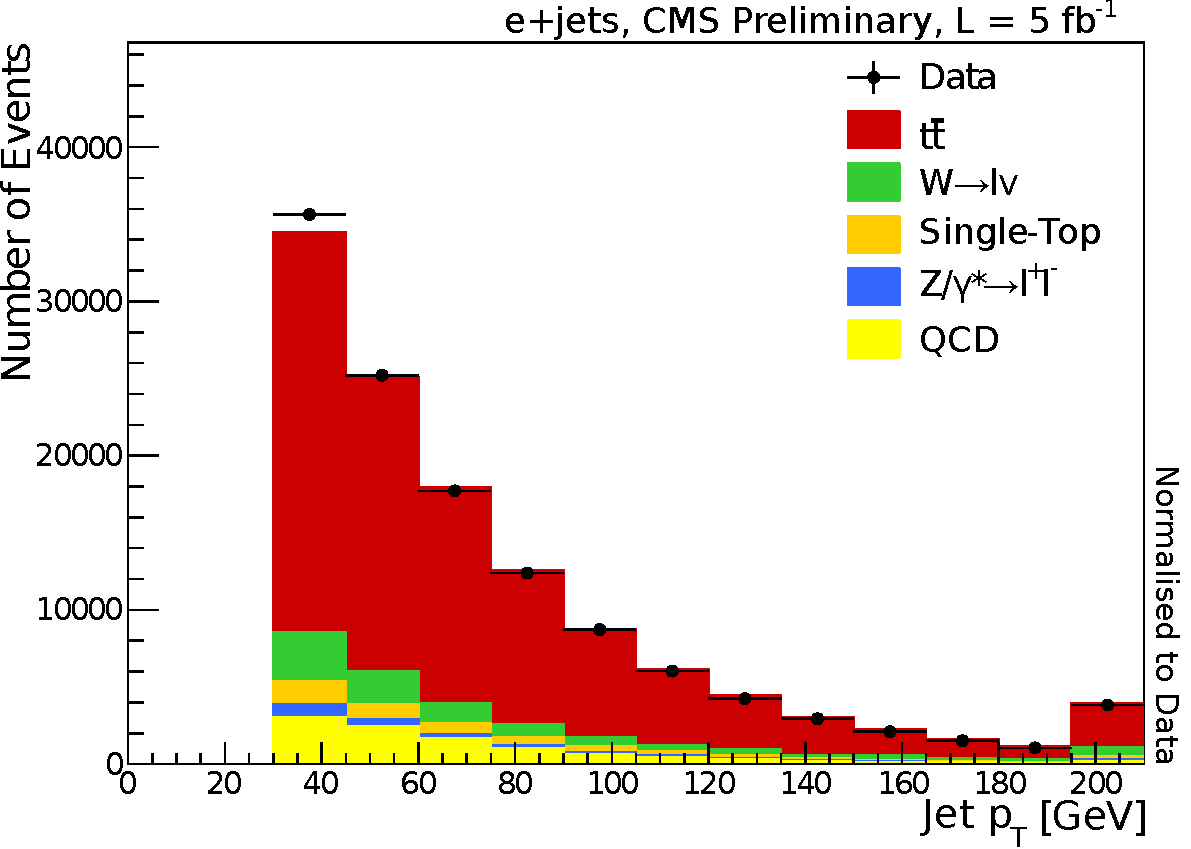
\includegraphics[width=0.5\textwidth]{cmg_jet_pt}}
   \subfloat[]{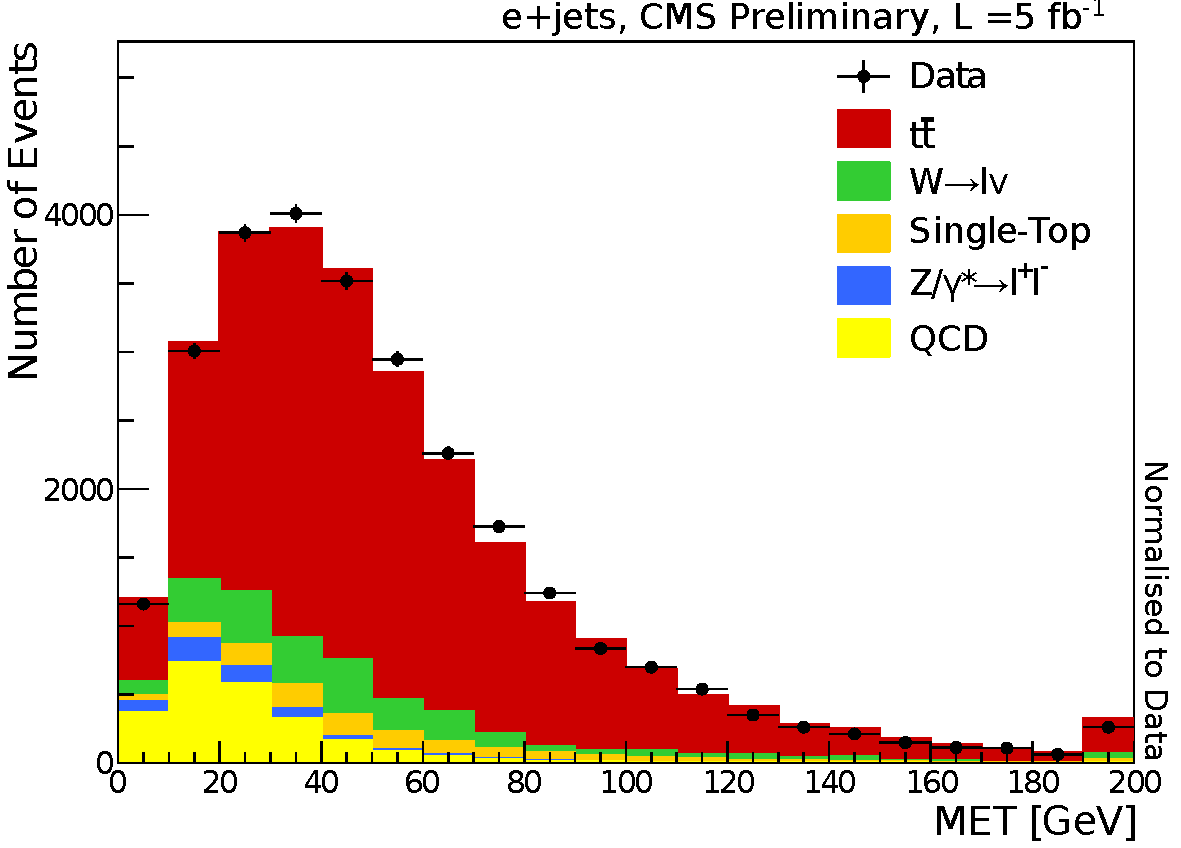
\includegraphics[width=0.5\textwidth]{cmg_met}}
   \caption{\label{fig:controlplots}Kinematic variable distributions after all selection cuts. (a) electron \pt, (b)
   electron $\eta$, (c) jet \pt for all jets passing the selection, (d) \MET.}
\end{figure}

\section{Kinematic Fit}
\label{s_top_mass:kinematic_fit}

In order to precisely measure the top quark mass, objects in the final state need to be associated with the originating
partons of the top quark pair decay. In this analysis, a kinematic fit is employed to fully reconstruct the event
kinematics under the \ttbar hypothesis, thus improving the resolution of measured quantities by exploiting the knowledge
of decay process.

The \HitFit fitting package \autocite{HitFit} used in this work originates from the \Dzero collaboration. Based on the
SQUAW algorithm \autocite{SQUAW} developed in Lawrence Berkeley National Laboratory, the original \HitFit code was
written by Scott Stuart Snyder in Fortran for Run I of the Tevatron. It was successfully used in the first direct
measurement of the top quark mass by \Dzero for lepton plus jets \ttbar events \autocite{D0_top_mass_1998}. The package
was then migrated to \Cplusplus for Run II of the Tevatron, and exploited in a series of \ttbar analyses including the
updated top quark mass measurement using the ideogram method \autocite{D0_top_mass_ljets_ideogram}, first measurement of
the forward-backward charge asymmetry in \ttbar production \autocite{D0_charge_assymetry} and some others.

One of the key features of the \HitFit package is its independence of specific experiments and detector geometries. The
only external dependence is on \textsc{CLHEP} \autocite{CLHEP}, a \Cplusplus library that provides utility classes for
linear algebra, geometry, vector arithmetic, etc., which was specifically developed for high energy physics simulation
and analysis software and is notably used by \GEANTfour package. In 2011 \HitFit was ported to CMSSW and later on
successfully used in a number of CMS top quark analyses, including the top mass measurement in the lepton plus jets
channel \autocite{top_mass_ljets_CMS}.

\HitFit is designed to fit lepton plus jets events under the \ttbar hypothesis. Specifically, it strives to constrain
the event to a hypothesis of production of two heavy particles, each decaying into a \W boson and \cPqb quark. According
to the semileptonic signature, one of the \W boson decays into an electron-neutrino pair, while the other decays into a
light quark-antiquark pair.

The input to the fit includes the four-momenta of the lepton, four leading jets and missing transverse energy, as well
as their respective resolutions that were calculated using Monte Carlo samples. Since only four leading jets are used,
there are $4!=24$ ways to associate these four reconstructed jets with the partons from the \ttbar decay. The number of
permutations is reduced to $4!/2=12$ since the light jets from the hadronic \W decay are interchangeable. However, for
each hypothesis the $z$ component of neutrino four-momentum needs to be determined. This is done by requiring the two
heavy particles to have equal mass ($m_{\cPqt} = m_{\cPaqt}$), which yields a quadratic equation which has either two
real solutions, or two complex solutions that share the real part. In the case of the two real solutions, the fit is
performed for each of them. If there are two complex solutions, the fit is performed once for the common real part of
them, but the fit result is included in the event content twice. Therefore, each hypothesis has two possible values of
the neutrino four-momentum, which doubles the number of permutations back to $4!=24$.

The kinematic fit is performed by minimising the $\chi^{2}$ function defined as
\begin{equation}
\chi^{2}  = (\mathbf{x} - \mathbf{x}^{m})^{T}\mathbf{G}(\mathbf{x} - \mathbf{x}^{m})
\end{equation}
where $\mathbf{x}^{m}$ is the vector or measured observables, $\mathbf{x}$ is the vector of fitted variables and
$\mathbf{G}$ is the inverse of the error matrix given by the resolutions of the observables.

The following kinematic constraints are imposed:
\begin{enumerate}[topsep=\parskip, parsep=\parskip, itemsep=\parskip, leftmargin=\leftmargin]
	\item Reconstructed top quarks from both hadronic and leptonic legs are required to have equal masses:
	\begin{equation}
		%m(t \to \ell \nu b) = m(\bar{t} \to q\bar{q} \bar{b}),
		m(\cPqt \to \ell \nu \cPqb) = m(\cPaqt \to \cPq\cPaq \cPaqb),
	\end{equation}
	\item The \W boson masses reconstructed in both hadronic and leptonic legs are fixed:
	\begin{equation}
		%m(\ell \nu) = m(q \bar{q}) = m_{W} = \SI{80.4}{\GeV}.
		m(\ell \nu) = m(\cPq\cPaq) = m_{\W} = \SI{80.4}{\GeV}.
	\end{equation}
\end{enumerate}

Apart from exploiting the knowledge of the \W mass, the \cPqb quark mass of \SI{4.7}{\GeV} is also used. Light quarks
and leptons are considered to be massless.

The full description of the fitting algorithm can be found in the appendix of the \HitFit author's PhD thesis
\autocite{Snyder}. Essentially, since the constraints are non-linear, an iterative technique is used. Starting with the
measured observables, the constraint equations are linearised by expansion in a power series around the starting point.
The minimisation is then solved with these linearised constraints, providing the new starting value for the next
minimisation step which is repeated until the $\chi^2$ converges or a maximum number of iterations is reached. Events
are rejected if there is no permutation resulting in a converging fit. Some kinematic variables for permutations giving
the best (smallest) $\chi^2$ values are shown in Figure~\ref{fig:fitplots}.

\begin{figure}[!htp]
   \centering
   \subfloat[]{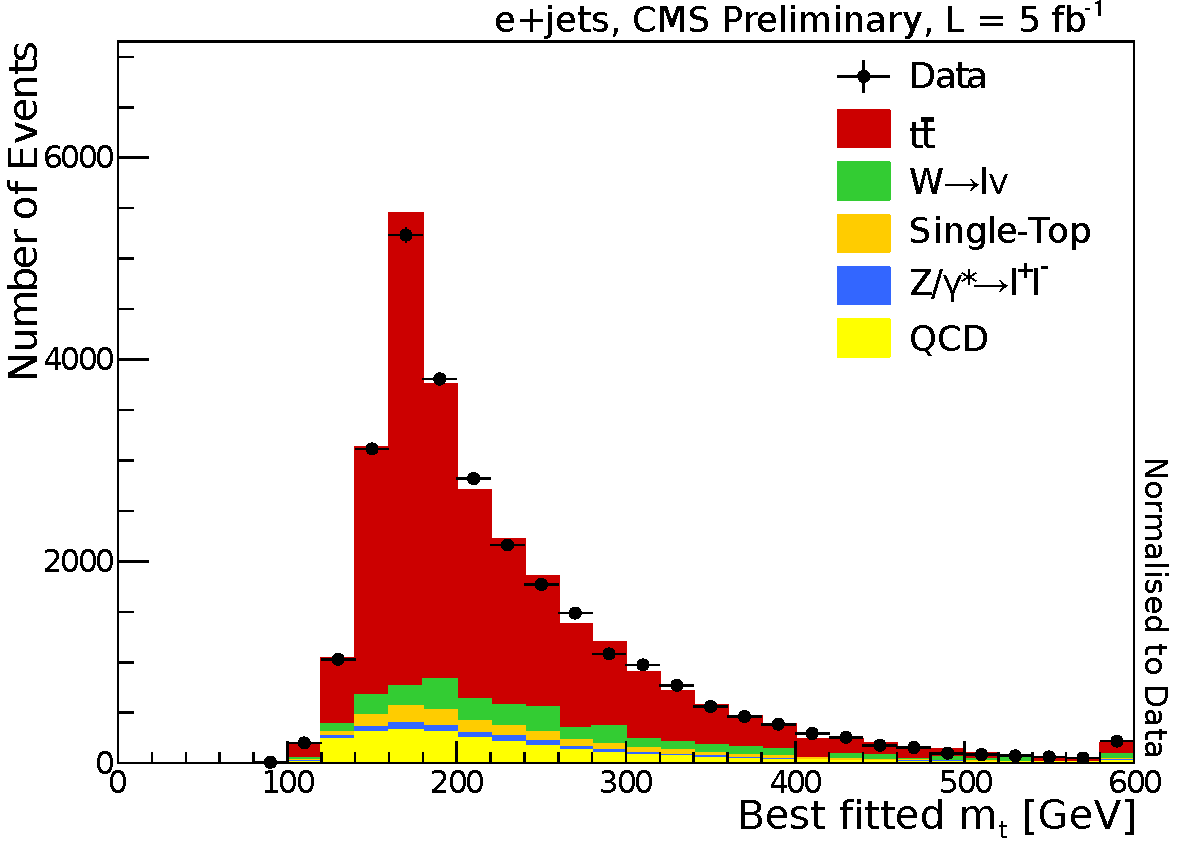
\includegraphics[width=0.5\textwidth]{hitfit_best_fitted_top_mass}}
   \subfloat[]{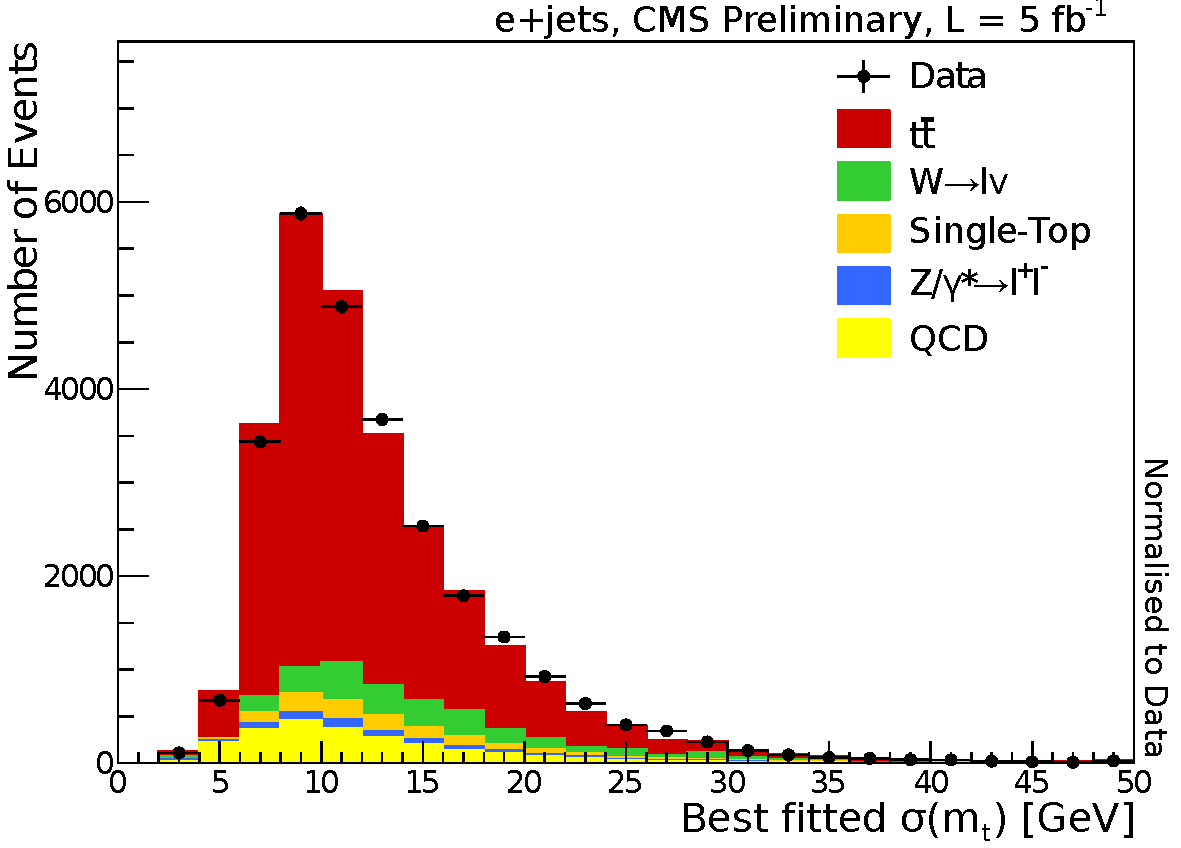
\includegraphics[width=0.5\textwidth]{hitfit_best_fitted_sigma_top_mass}}
   \hfill
   \subfloat[]{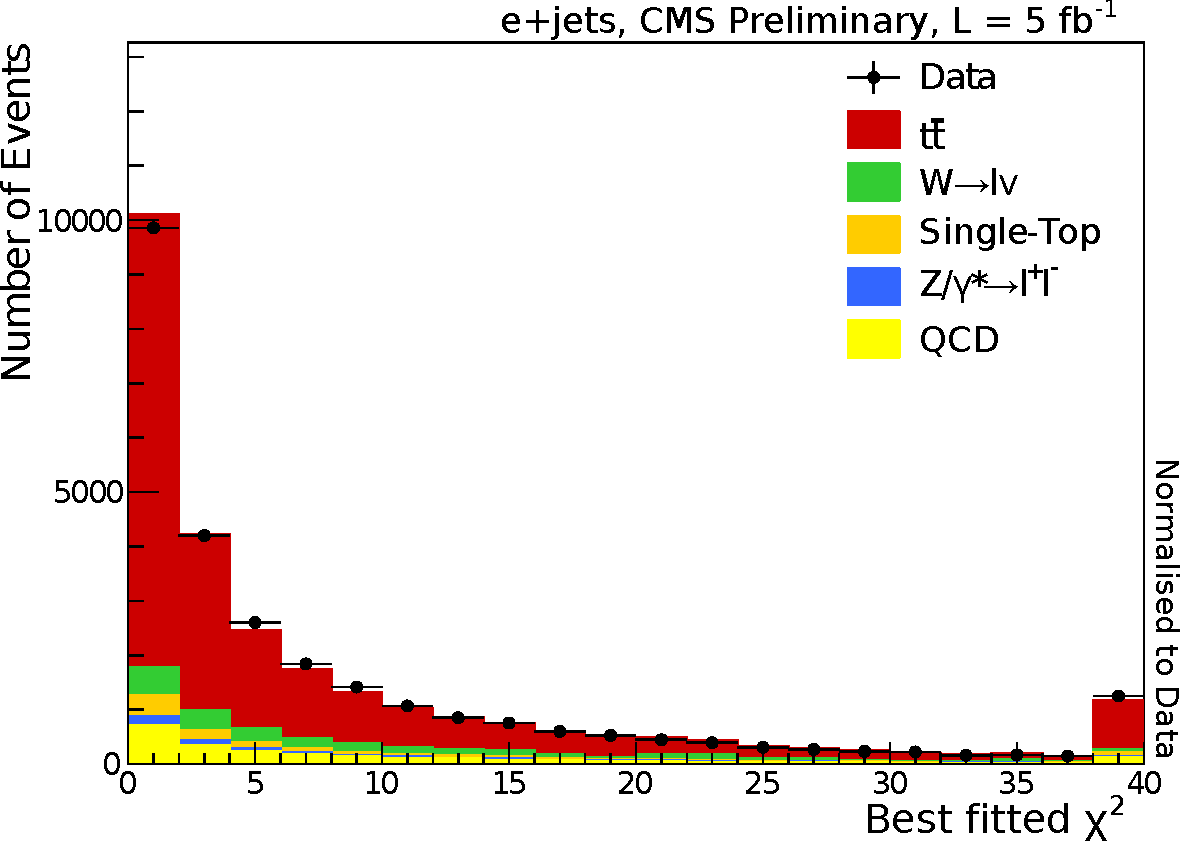
\includegraphics[width=0.5\textwidth]{hitfit_best_fitted_chi2}}
   \subfloat[]{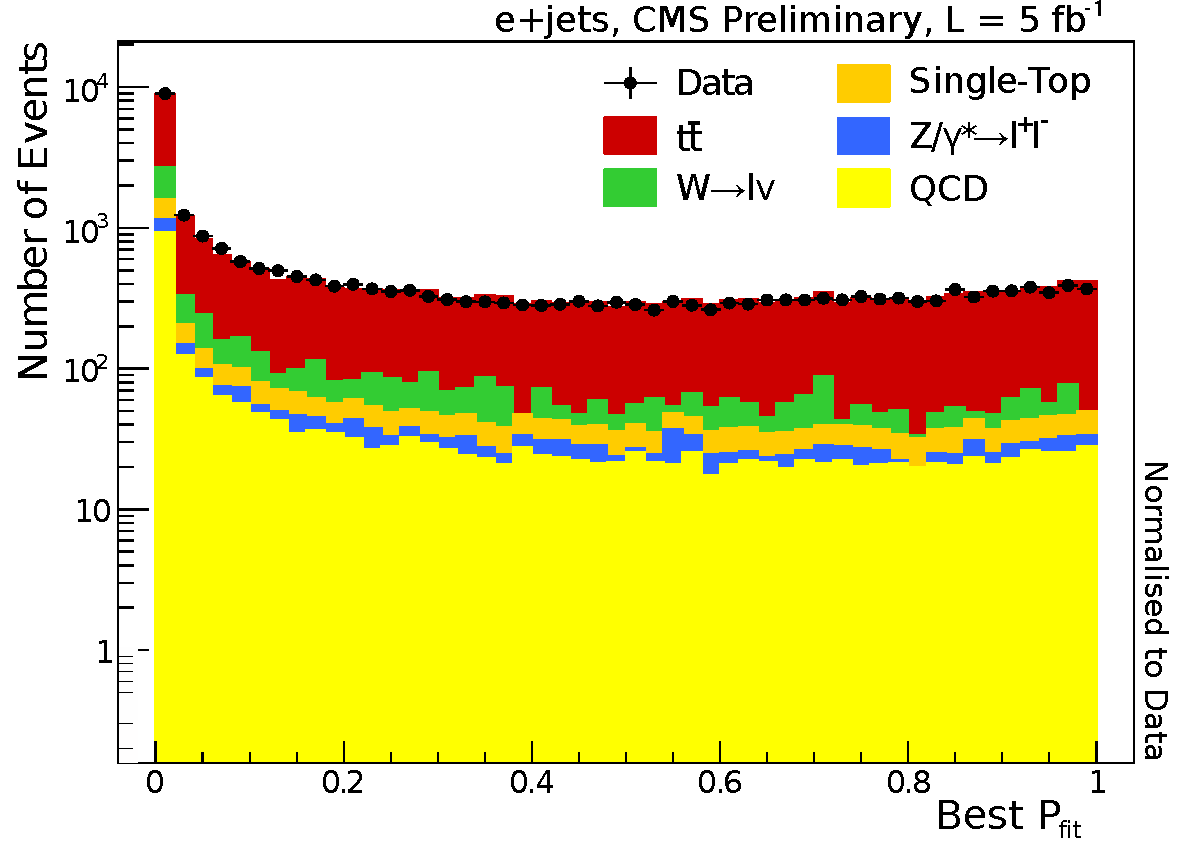
\includegraphics[width=0.5\textwidth]{hitfit_best_pfit}}
   \caption{\label{fig:fitplots}Distribution of (a) fitted top quark mass, (b) its standard deviation, (c) $\chi^{2}$
   and (d) fit probability for the best fitted hypotheses.}
\end{figure}

Typically, an event has a few permutations resulting in a converged fit. The simplest approach of picking a permutation
with the best $\chi^2$ value is disfavoured, since Monte Carlo studies have shown that the correct permutation does not
necessarily have the best $\chi^2$ \autocite{Snyder}. This value can change drastically with relatively small variations
of the input parameters, as different permutations may obtain the smallest value of $\chi^2$. On the other hand, some
solutions yield very large $\chi^2$ value, which typically happens for badly reconstructed or background events.
Therefore, a loose cut of $\chi^2=20$ is applied for all permutations on the output of the converged fit. This is the
final selection criterion on top of the reference selection mentioned in Section~\ref{s_top_mass:event_selection}.

%Table \ref{tab:chi2_eff} list the number of events which pass the reference selection only, and number of events which
% pass both the reference selection and the loose $\chi^{2}$ cut.

The compatibility of a permutation with the \ttbar hypothesis is quantified by the following fit probability:
\begin{equation}
	P_{\textrm{fit}} = \textrm{exp}(-\frac{1}{2}\chi^2).
	\label{eq:fit_probability}
\end{equation}

This probability is used in the next step of the analysis, referred to as the ideogram method.

\section{The Ideogram Method}
\label{s_top_mass:ideogram_method}

The ideogram method is a powerful mass extraction technique. Its main idea lies in finding the likelihood distribution
of the particle mass given the particular data sample, which is performed by evaluating the likelihood of measured
observables given a generated particle mass for each event in the sample. The signal likelihood is evaluated from the
theoretically expected Breit-Wigner distribution convoluted with the Gaussian experimental resolution on event-by-event
basis. The whole procedure is calibrated using Monte Carlo simulation of a series of particle masses in the expected
region.

%All selected jet-parton permutations from the output of the kinematic fit are weighted by their fit probability
%$P_{\textrm{fit}}$.

One of the first applications of the ideogram method tracks back to the \W boson mass measurement by the \textsc{DELPHI}
Collaboration at CERN LEP collider \autocite{DELPHI_1998, DELPHI_2008}. It was later used in a series of top quark mass
measurements, including the \Dzero measurement in the lepton plus jets channel \autocite{D0_top_mass_ljets_ideogram} and
CDF measurement in the all-hadronic channel \autocite{CDF_ideogram}. The main CMS top quark mass measurement in lepton
plus jets channel at \SI{7}{\TeV} \autocite{top_mass_ljets_CMS} which is cross-checked by this analysis is also based on
the ideogram method with, however, \textit{in situ} JES (jet energy scale) measurement in a joint likelihood fit. As JES
is a dominant systematic in this analysis, this approach proved to be more precise, but let us not neglect the
importance of a cross-check.

\subsection{Event likelihood}
\label{ss_top_mass:event_likelihood}

In the basis of the ideogram method lies the event likelihood, also referred to as the ideogram. It is calculated for
each event in the sample as a function of the hypothesised top quark mass \mtop in the following way:

\begin{equation}
\mathcal{L}_\textrm{event} \left(\mathbf{x}|\mtop, f_{\ttbar} \right) = f_{\ttbar} P_{\ttbar}
\left(\mathbf{x}|\mtop\right) + \left(1 - f_{\ttbar} \right)P_\textrm{bkg}\left(\mathbf{x}\right).
\label{eq:event_likelihood}
\end{equation}

Here $\mathbf{x}$ is the set of event observables with the top mass information from the kinematic fit, $f_{\ttbar}$ is
the fraction of \ttbar events in the data sample, and $P_{\ttbar}$ and $P_\textrm{bkg}$ are probability densities for
signal and background events, respectively. Essentially, by construction of the likelihood, the first term corresponds
to the probability for the event to be signal, whilst the second term is its probability to be background. The kinematic
information $\mathbf{x}$ includes the fitted mass $m_{i}$, the estimated standard deviation for each fitted mass
$\sigma(m_{i})$ and the goodness-of-fit $\chi^{2}_{i}$ for all permutations, i.e.\ all possible jet-parton assignments
and neutrino solutions surviving the selection criteria on the output of the fit.

\subsubsection*{Jet-parton assignment weights}
The signal and background probabilities forming the event likelihood are calculated as a weighted sum over jet-parton
assignments and neutrino solutions coming from the kinematic fit. Each permutation is weighted by the probability that
it is correct, which is essentially the fit probability $P_{\textrm{fit}}$ introduced in
Equation~\ref{eq:fit_probability}. However, this particular implementation of the ideogram method also exploits the
b-tagging information, thus the fit probability is multiplied by an additional term $p_{\rm btags}$, which is the
probability that the particular jet-parton assignment is compatible with the observed b-tags:

\begin{equation}
p_{\rm btags} = \prod_{j=1}^{4} p^{j}
\end{equation}

Here the index $j$ runs over all four jets in the kinematic fit, and the probability $p^{j}$ can be either
$\varepsilon_{l}$, $(1 - \varepsilon_{l})$, $\varepsilon_{b}$, or $(1 - \varepsilon_{b})$, depending on the flavour of
the jet as derived by the fit (light jet or \cPqb-jet), and whether the jet is b-tagged or not. As a recap from
Section~\ref{sss:b-tagging}, for the medium working point of CSV b-tagging algorithm used in this analysis, b-tagging
efficiency is approximately \SI{\sim70}{\percent}, whilst the mis-tag rate (or $(1 - \varepsilon_{l})$) is approximately
\SI{1}{\percent}.

Therefore, for each such permutation the relative weight is $w_i$ is calculated as:

\begin{equation}
w_i = p_{\rm fit} \cdot p_{\rm btags} = \textrm{exp}(-\frac{1}{2}\chi^2) \cdot \prod_{j=1}^{4} p^{j}
\label{eq:permutation_weight}
\end{equation}

These weights are used in the calculation of signal and background probability densities, described hereafter.

\subsubsection*{Signal probability}

The \ttbar signal probability in the event likelihood shown in Equation~\ref{eq:event_likelihood} is calculated as a
weighted sum over all permutations:
\begin{equation}
P_{\ttbar}\left(\mathbf{x}|\mtop\right) = \sum_{i}^{24} w_{i} \left( f_{\textrm{cp}} \cdot
\int\limits^{m_{\textrm{max}}}_{m_{\textrm{min}}} \textrm{G}\left(m'|m_{i},\sigma_{i}\right) \textrm{RBW}
\left(m'|\mtop,\Gamma_{\textrm{t}}\right) \textrm{d}m' + (1 - f_{\textrm{cp}})\textrm{WP}(m_{i}|\mtop)\right)
\end{equation}

Here $f_{\textrm{cp}}$ is the fraction of events in which the maximum weight is assigned to the correct permutation,
estimated from simulated \ttbar events. For each permutation, the first term expresses the probability that it has a
correct jet-parton assignment (correct permutation). It is calculated as a convolution of a relativistic Breit-Wigner
distribution $\textrm{RBW}(m'|\mtop,\Gamma_{\textrm{t}})$ and a Gaussian $\textrm{G}(m'|m_{i},\sigma_{i})$.

The relativistic Breit-Wigner distribution describes the theoretical top quark mass distribution for a given
hypothesised top quark mass value \mtop with a top quark width $\Gamma_{\textrm{t}}$ set to \SI{2}{\GeV}, according to
the latest experimental results \autocite{top_width_D0}. As suggested by Standard Model electroweak corrections and
$s-$dependence of the phase space \cite{aleph_Z_RBW}, the following form of RBW is used:
\begin{equation}
\textrm{RBW}(m'|\mtop,\Gamma_{\textrm{t}}) \propto \frac{{m'}^{2}}{\left({m'}^{2} - {\mtop}^{2}
\right)^{2} + {m'}^{4}\frac{\Gamma_{\textrm{t}}}{{\mtop}^{2}}}
\end{equation}
%need to properly understand

The Gaussian in the convolution represents the detector resolution. It is centred at the fitted mass value $m_{i}$ with
a width of the fitted mass uncertainty $\sigma_{i}$ as estimated by the fit:

\begin{equation}
\textrm{G}(m'|m_{i},\sigma_{i}) = \frac{1}{\sigma_{i}\sqrt{2\pi}}
\textrm{exp}\left(\frac{(m'-m_{i})^{2}}{2\sigma_{i}^2}\right)
\end{equation}

The resulting probability density for \ttbar events with correct permutations is shown in
Figure~\ref{fig:fitted_ttbar_cp_density}. The Monte Carlo sample with top mass of \SI{166.5}{\GeV} was used, for
illustration.

\begin{figure}[!htpb]
	\centering
    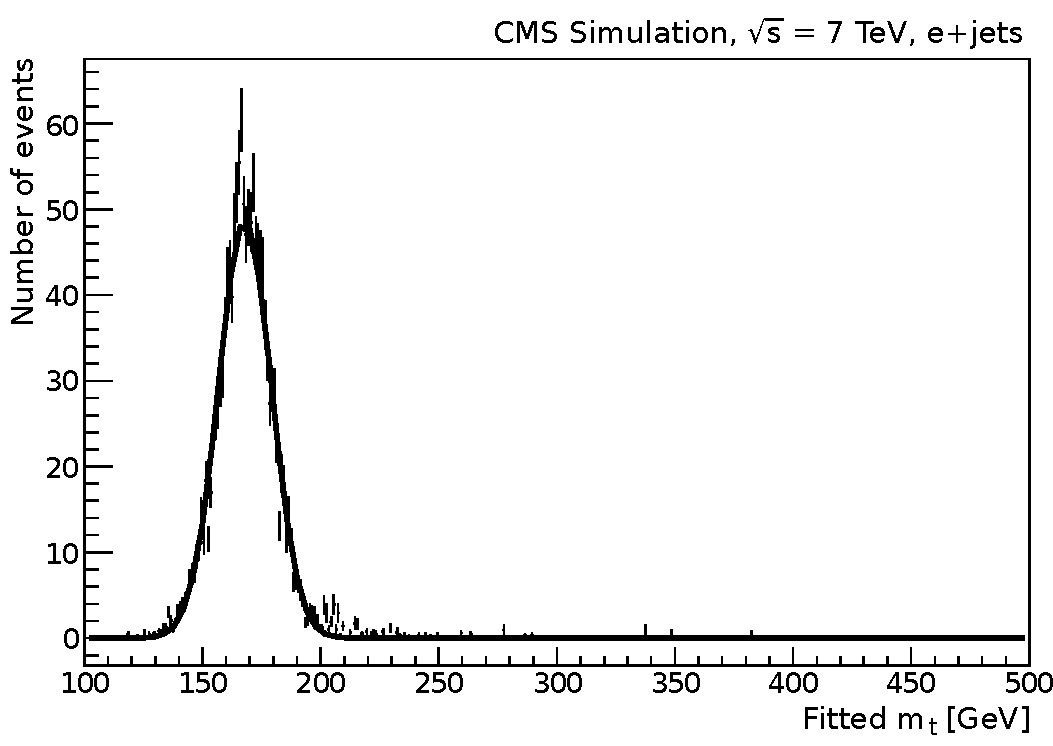
\includegraphics[width=0.65\textwidth]{correct_permutations_fitted_top_mass}
	\caption{\label{fig:fitted_ttbar_cp_density}
	The fitted top quark mass distribution for \ttbar events with correct permutations (MC truth, \mtop =
	\SI{166.5}{\GeV}).}
\end{figure}

The second term shows the probability of a wrong permutation in the signal event. This probability density, denoted
$\textrm{WP}(m_i|\mtop)$, is calculated by fitting the Crystal Ball analytical function to the fitted top quark mass
distribution for permutations with wrong jet-parton assignment, estimated purely from Monte Carlo \ttbar sample whilst
taking the permutation weights (Equation~\ref{eq:permutation_weight}) into account. The wrong permutations fall in two
categories: the first one corresponds to events where the four leading jets come from \ttbar decay, but are not assigned
to the partons correctly; the second one are events with one ore more of the four leading jets coming from soft gluon
radiation (ISR or FSR). It was found that the fitted top quark mass distributions have similar shapes for both
categories, therefore they were combined for the purpose of fitting. The Crystal Ball function has the form of:

\begin{equation}
\textrm{CB}(x;\mu,\sigma,\alpha,n) = N \times
\begin{cases}
\frac{1}{\sqrt{2\pi\sigma}}\exp(-\frac{(x-\mu)^2}{2\sigma^2}) & \text{if $\frac{x-\mu}{\sigma} > -\alpha$,} \\
\frac{1}{\sqrt{2\pi\sigma}}(\frac{n}{|\alpha|})^n
\exp(-\frac{|\alpha|^2}{2})(\frac{n}{|\alpha|}-|\alpha|-\frac{x-\mu}{\sigma})^{-n} & \text{if $\frac{x-\mu}{\sigma}
\leq -\alpha$.}
\end{cases}
\label{eq:crystal_ball}
\end{equation}

The exponential order of $n=\num{5}$ was used, and parameters $\mu$, $\sigma$, and $\alpha$ were parametrised as
functions of the top quark mass. The fitted distributions of wrong permutations spectra for three different top masses
(\SIlist{166.5;172.5;178.5}{\GeV}) are shown in Figure \ref{fig:fitted_ttbar_wp_density}.

\begin{figure}[!htpb]
	\centering
	\subfloat[]{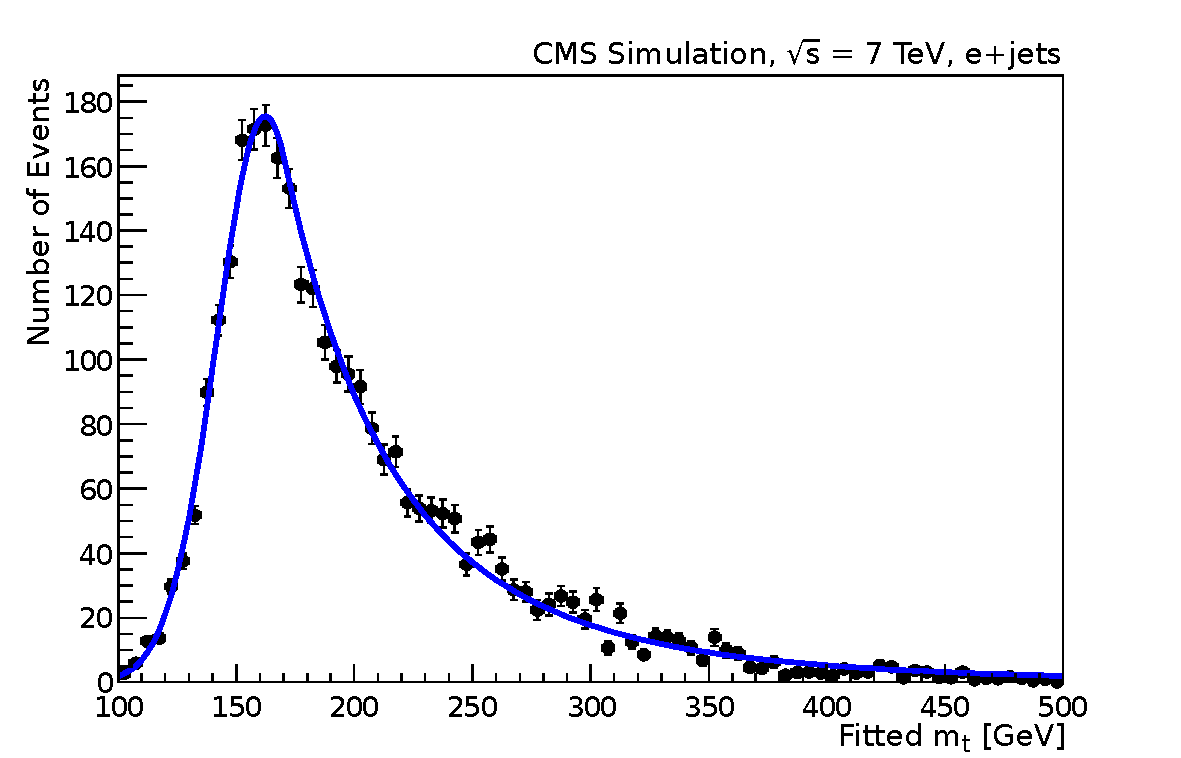
\includegraphics[width=0.50\textwidth]{wrong_permutations_fitted_top_mass_166}}
	\subfloat[]{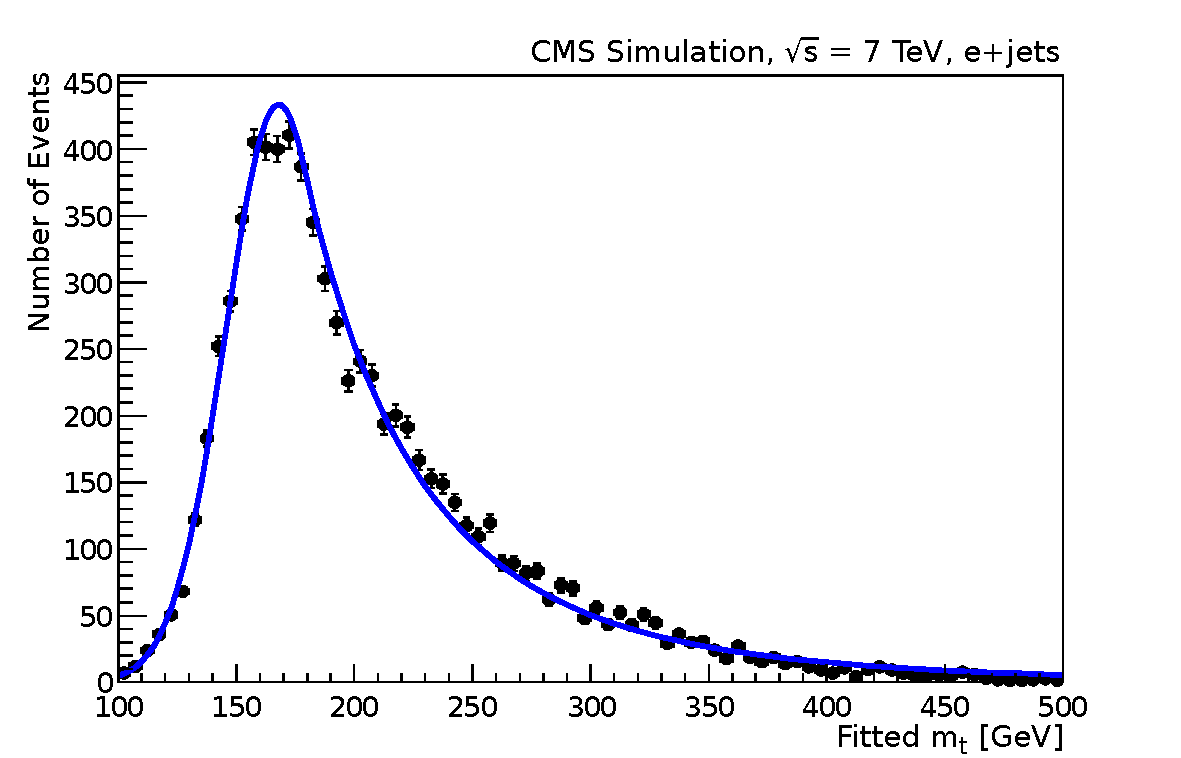
\includegraphics[width=0.50\textwidth]{wrong_permutations_fitted_top_mass_172}}
	\hfill
	\subfloat[]{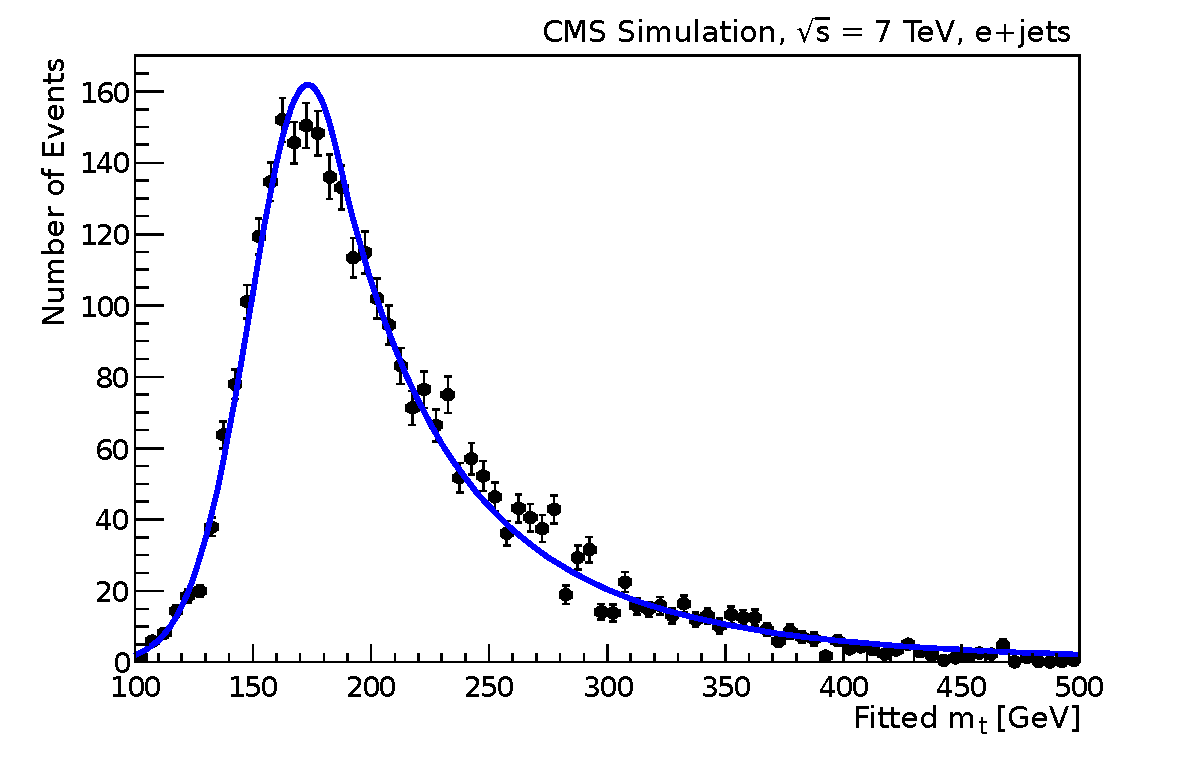
\includegraphics[width=0.50\textwidth]{wrong_permutations_fitted_top_mass_178}}
	\caption{\label{fig:fitted_ttbar_wp_density}
	The fitted top quark mass distribution for \ttbar events with wrong permutations (MC truth) for (a)
	$\mtop=\SI{166.5}{\GeV}$, (b) $\mtop=\SI{172.5}{\GeV}$, (c) $\mtop=\SI{178.5}{\GeV}$.}
\end{figure}

\subsubsection*{Background probability}

The shape of the background probability density in Equation~\ref{eq:event_likelihood} is assumed not to depend on the
top quark mass, and is estimated from the background Monte Carlo samples. The procedure is done in a similar way to the
wrong permutations probability, and the jet-parton assignment weights (Equation~\ref{eq:permutation_weight}) are also
taken into account. Since the dominant background is \WpJets, it was used exclusively for extracting the fitted top
quark mass distribution by running the kinematic fit. The contribution from single top, \ZpJets and QCD was expected to
be small, and it was confirmed that their probability density distributions have similar shapes to that of the \WpJets
sample. Moreover, the Monte Carlo calibration described later on in Section~\ref{s_top_mass:calibration} takes all
mentioned background sources into account, therefore any possible bias due to this approximation is corrected for.

The fitted top quark mass spectrum for background events as estimated from the \WpJets MC sample is shown in
Figure~\ref{fig:background_wjets_fitted_top_mass}. This distribution is described by the Landau function, fitted by the
\ROOT package \autocite{Landau}.
% \begin{equation}
% \textrm{L}(x) = \frac{1}{\sqrt{2\pi}}\exp\left(-\frac{1}{2}(x+e^{-x})\right).
% \label{eq:landau}
% \end{equation}

\begin{figure}[!htpb]
	\centering
	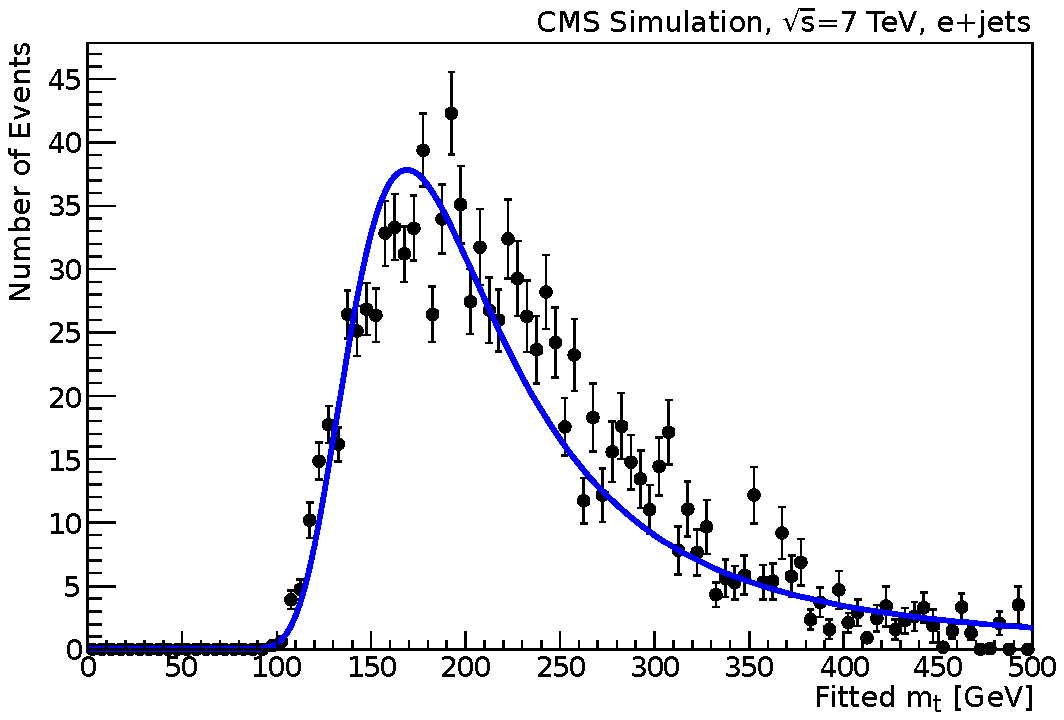
\includegraphics[width=0.65\textwidth]{background_wjets_fitted_top_mass}
	\caption{\label{fig:background_wjets_fitted_top_mass}
	The fitted top quark mass distribution for \ttbar events in \WpJets Monte Carlo sample.}
\end{figure}

\subsection{Combined likelihood fit}
\label{ss_top_mass:likelihood_fit}

Finally, for the extraction of the top quark mass the total likelihood for the entire data sample is calculated as the
product of all the event likelihoods:
\begin{equation}
\mathcal{L}_{\rm sample} = \prod_{\rm all~events}
\mathcal{L}_\textrm{event} \left(\mathbf{x}|\mtop \right)
\label{eq:CombinedLikelihood}
\end{equation}

To extract the most probable top quark mass, this likelihood needs to be maximised. In practice, it is simplified by
performing the minimisation of the summed negative log-likelihoods:

\begin{equation}
 -2\log{\mathcal{L}_{\rm sample}} = -2 \sum_{\rm all~events} \log{\mathcal{L}_\textrm{event} \left(\mathbf{x}|\mtop
 \right)}
\label{eq:CombinedLogLikelihood}
\end{equation}

The result with the full dataset is shown in Figure~\ref{fig:LogLikelihood}. The top quark mass and its statistical
uncertainty are calculated by using the parabolic interpolation with three lowest points in the log-likelihood curve.
However, this result can not be regarded as the final measurement, as it does not take into account the possible mass
bias of the ideogram method. The mass calibration technique is described in the next section.

\begin{figure}[!htpb]
	\centering
	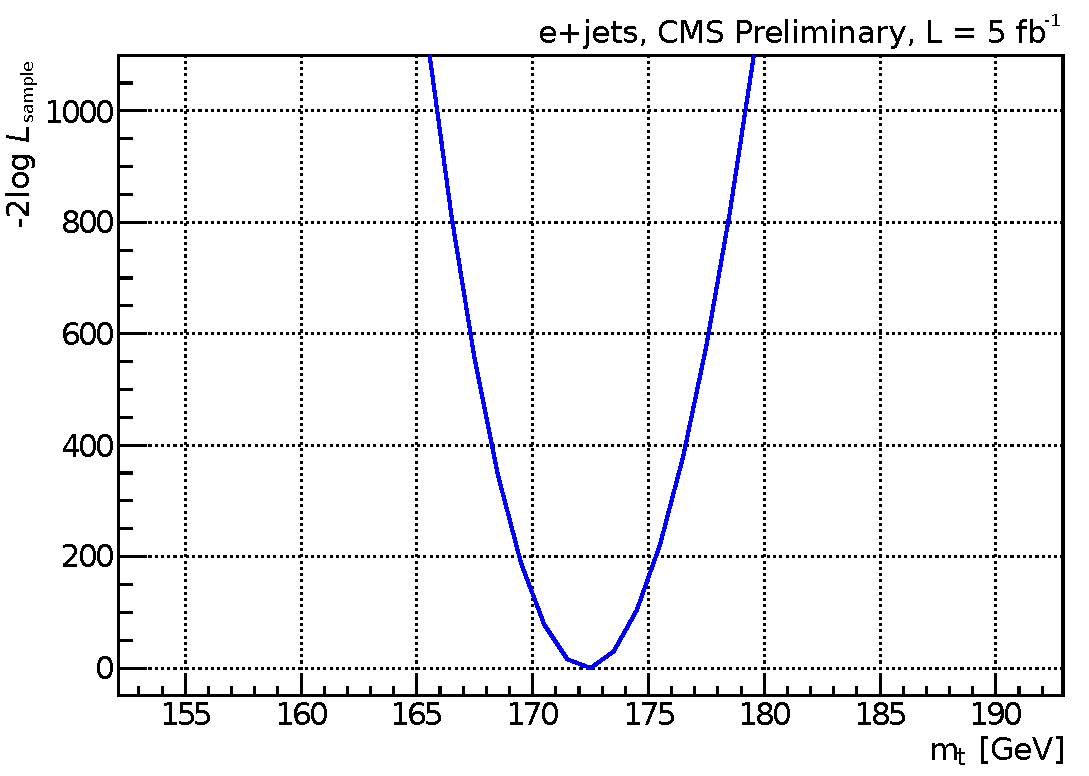
\includegraphics[width=0.65\textwidth]{Likelihood}
	\caption{\label{fig:LogLikelihood}
	Log-likelihood curve as a function of top quark mass for e+jets dataset before calibration.}
\end{figure}

\section{Mass Calibration}
\label{s_top_mass:calibration}

By construction of the ideogram method, it has approximations which can lead to possible bias in the top quark mass
measurement. To account for this bias, a calibration is performed by running the measurement on Monte Carlo simulation
with known true top quark mass. Pseudo-experiments are used to measure the bias in the fitted mass, as well as to
calibrate the statistical uncertainty of the measurement.

For each of the nine generated \ttbar samples with mass points between \SI{161.5}{\GeV} and \SI{184.5}{\GeV},
\num{5000} pseudo-experiments were performed with events picked from Monte Carlo samples representing different sources
of events, so that the numbers of events follow a Poisson distribution centred around the corresponding numbers observed
in real data. The observed value of \num{23727} electron plus jets events with an average signal fraction of
\SI{76}{\pc} was used in each pseudo-experiment. The background was estimated by using events from the \WpJets MC
sample, whereas the impact of other background sources was accounted for separately as a systematic uncertainty
(Section~\ref{s_top_mass:systematics}). For every pseudo-experiment all the event likelihoods are calculated, the total
log-likelihood is formed and the top quark mass ($m_i$) with its statistical uncertainty ($\sigma_i$) are extracted in
the same way as in the real measurement described above. These results are used to derive the bias and pull
distributions, defined as follows:
\begin{equation}
 \textrm{bias} = \mtop^{\rm meas} - \mtop^{\rm gen} \quad \text{and} \quad
 \textrm{pull}_i = \frac{m_i - \mtop^{\rm meas}}{\sigma_i},
\label{eq:bias_pull}
\end{equation}
where $\mtop^{\rm meas}$ is the mean top quark mass over all pseudo-experiments, for a given generated mass point. The
width of the pull is defined as the standard deviation of a Gaussian fitted to the pull distribution.

The mass bias and the width of the pull as a function of the generated top quark mass are shown in
Figure~\ref{fig:bias_pull_vs_mass}. Clearly, using the ideogram method out of the box reveals a significant bias which
needs to be corrected for. It can also be seen that the width of the pull distribution is approximately \SI{11}{\pc}
larger than unity, suggesting that the ideogram method underestimates the statistical uncertainty.

%why is the mass bias linear with the true top mass? How exactly is calibration applied?

\begin{figure}[!htp]
   \subfloat[]{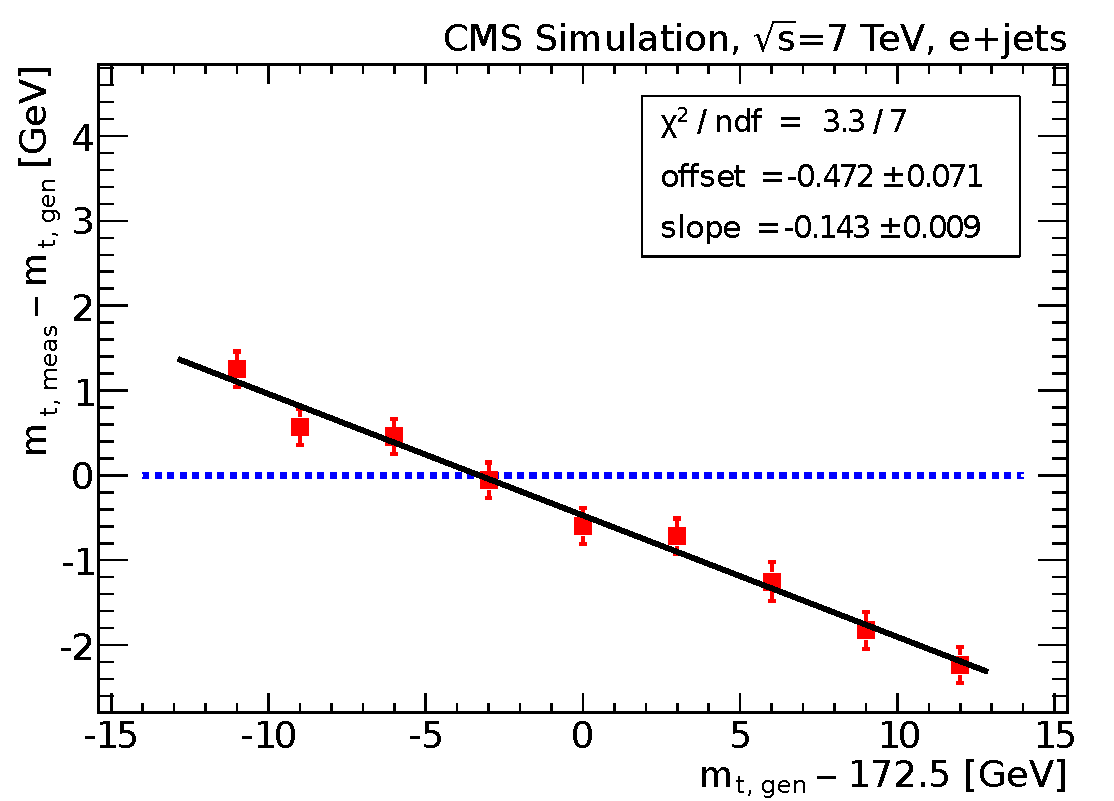
\includegraphics[width=0.485\textwidth]{bias}}
   \subfloat[]{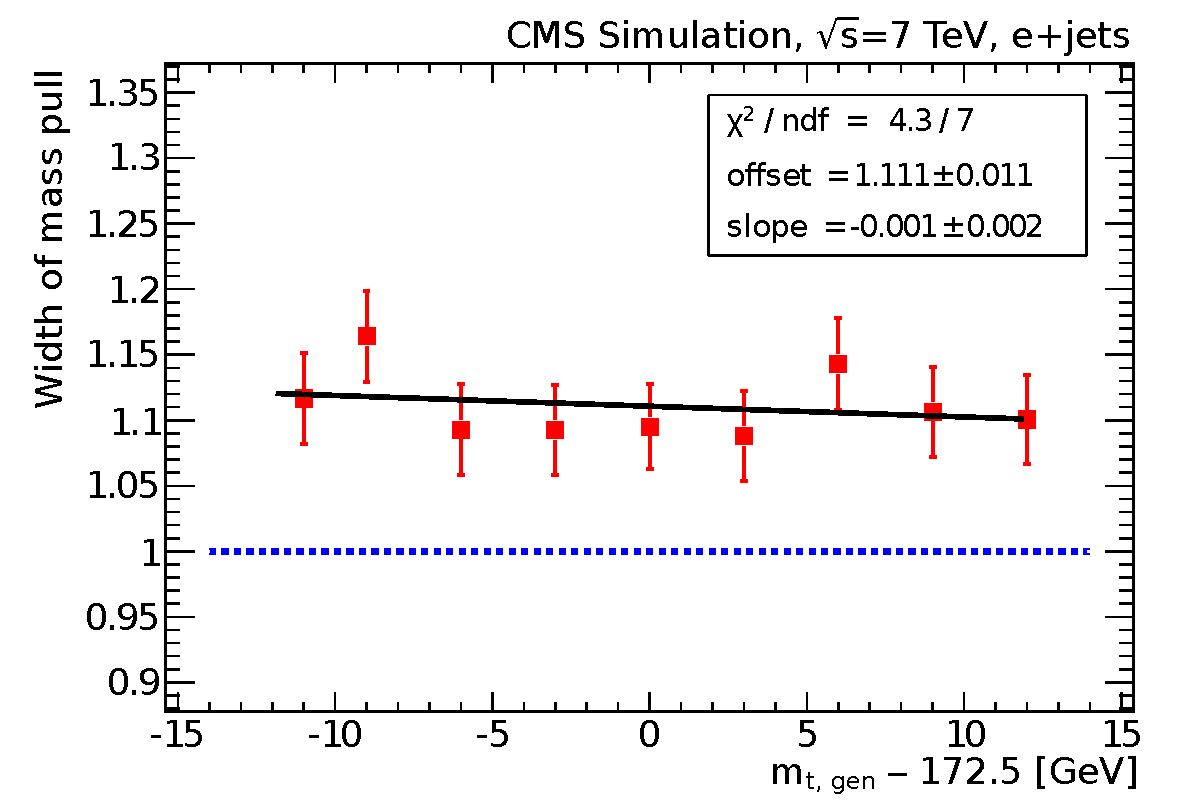
\includegraphics[width=0.515\textwidth]{pull}}
   \caption{Average mass bias (a) and width of the pull (b) as a function of true top quark mass.
   \label{fig:bias_pull_vs_mass}}
\end{figure}

Due to the apparent bias, the fitted linear calibration curves in both distributions are used to correct the final
measurement of the top quark mass. As a closure test, the mass bias and pull width as a function of true top quark mass
are calculated after applying the full calibration. The distributions are shown in
Figure~\ref{fig:calibrated_bias_pull_vs_mass}. Evidently, the closure tests confirm that the top quark mass and its
statistical uncertainty are unbiased after calibration.

\begin{figure}[!htp]
   \subfloat[]{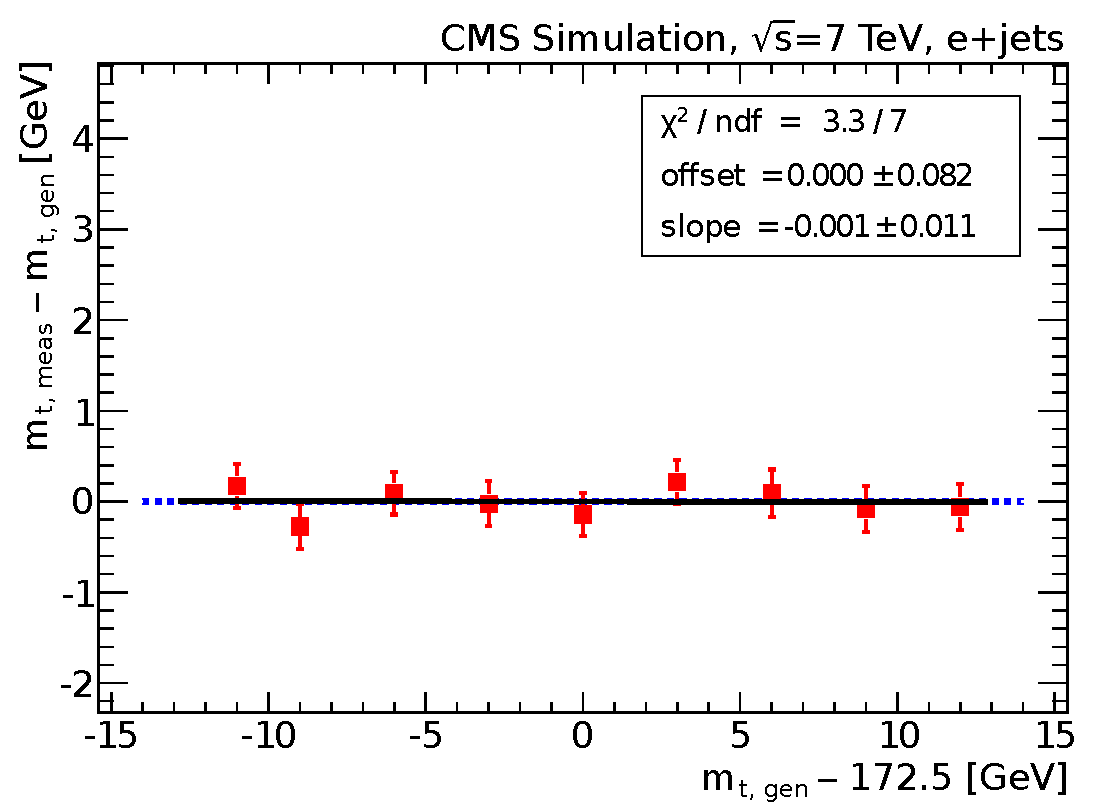
\includegraphics[width=0.485\textwidth]{bias_calibrated}}
   \subfloat[]{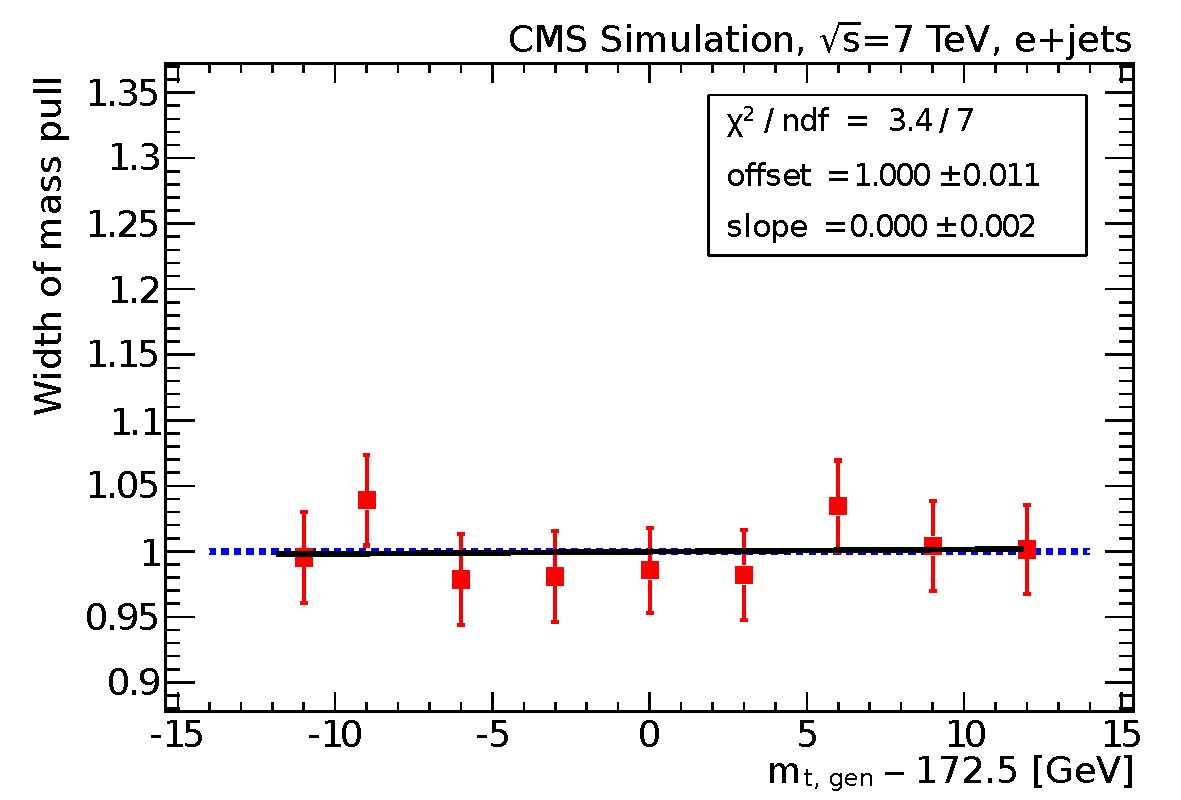
\includegraphics[width=0.515\textwidth]{pull_calibrated}}
   \caption{Closure test, showing the average mass bias (a) and width of the pull (b) as a function of true top quark
            mass after calibration.
   \label{fig:calibrated_bias_pull_vs_mass}}
\end{figure}
 

\section{Systematic Uncertainties}
\label{s_top_mass:systematics}

Like any measurement, the top quark mass measurement is prone to various systematic errors. In attempt to evaluate them,
several sources of systematic effects are considered in this analysis. These include theoretical uncertainties on Monte
Carlo modelling, assumptions made within the ideogram method, as well as imperfect understanding of detector effects and
reconstruction algorithms.

Systematic uncertainties are calculated by running the analysis with tuned MC samples where systematic effects are
varied by $\pm 1$ standard deviation, and comparing the result with the nominal one. The obtained difference in fitted
$\Delta \mtop$ is regarded as an uncertainty due to a given systematic effect. The total systematic error is calculated
as a sum of all components in quadrature, under the assumption that all the effects are uncorrelated. A summary of all
systematic uncertainties is given in Table~\ref{tab:top_mass_systematics}, whereas all corresponding sources are
described below.

% Since some of these systematic effects introduce very small shifts on the estimated top-quark mass, the statistical
% uncertainty of these induced shifts is calculated for every systematic effect.
% https://indico.cern.ch/getFile.py/access?subContId=1&contribId=1&resId=0&materialId=slides&confId=191766
% https://indico.cern.ch/getFile.py/access?subContId=0&contribId=2&resId=0&materialId=slides&confId=200007

\begin{table}[!htp]
\begin{center}
%\begin{tabular}{l|c|c|c}
\begin{tabular}{l|c}
\hline\hline
%                                   & \multicolumn{3}{c}{$\delta m_{\rm top}$ (GeV)}  \\
%\cline{2-4}
%Source of systematic effect        & $\mu$+jets  &  e+jets&  $\ell$+jets\\
%\hline
%Fit calibration statistics         & 0.10  & 0.12 & 0.07 \\
%$b$-tagging                        & 0.06  & 0.10 & 0.07 \\
%Jet Energy Scale (overall data/MC) & 1.20  & 1.21 & 1.21 \\
%%light vs b-jet scale               &	 &   &  \\
%Jet Energy Resolution              & 0.07  & NA   & NA   \\
%%MET (10 \% effect)                 &  \\
%Factorization scale                & 0.95  & 1.38 & 0.96 \\
%ME-PS matching threshold           & 0.83  & 0.93 & 0.61 \\
%Colour Reconnection                & 0.03  & 0.03 & 0.03 \\
%%ISR/FSR                            &  \\
%%Underlying event                   &  \\
%Non $t\bar{t}$ background          & 0.36  & 0.61 & 0.46 \\
%Pile up                            & 0.28  & 0.22 & 0.26 \\
%PDF                                & 0.17  & 0.15 & 0.16 \\
%\hline
%Total                              & 1.81  & 2.17 & 1.75 \\
                                   & $\delta m_{\rm top}$ (GeV)  \\
Source of systematic effect        & $\ell$+jets\\
\hline
Fit calibration statistics         & 0.13 \\
$b$-tagging                        & 0.07 \\
Jet Energy Scale (overall data/MC including b-JES) & 0.93 \\
%light vs b-jet scale               &	 &   &  \\
Jet Energy Resolution              & 0.07  \\
%MET (10 \% effect)                 &  \\
Factorization scale                & 0.94 \\
ME-PS matching threshold           & 0.40 \\
Colour Reconnection                & 0.07 \\
%ISR/FSR                            &  \\
Underlying event                   & 0.08 \\
Normalization of background        & 0.28 \\
Non $t\bar{t}$ background shape    & 0.32 \\
Pile up                            & 0.26 \\
PDF                                & 0.16 \\
\hline
Total                              & 1.49 \\
\hline\hline
\end{tabular}
\caption{\label{tab:systematics}Overview of systematic uncertainties
and their effect on the top mass measurement, split into various sources.}
\end{center}
\end{table}


\begin{table}[!htp]
\begin{center}
\begin{tabular}{l|c|c}
\hline\hline
$\Delta m_{\textrm{top}}$ (GeV)        & up  & down\\
\hline
$t \bar t$      & -0.78  $\pm$ 0.10 & 0.94 $\pm$ 0.10 \\
$W$+jets        & -0.525 $\pm$ 0.14 & -0.22 $\pm$ 0.14 \\
\hline\hline
\end{tabular}
\caption{\label{tab:systematicsScale}Individual variations due to $Q^2$ scale.}
\end{center}
\end{table}


\begin{table}[!htp]
\begin{center}
\begin{tabular}{l|c|c}
\hline\hline
$\Delta m_{\textrm{top}}$ (GeV)        & up  & down\\
\hline
$t \bar t$   &0.185 $\pm$ 0.103 & --- \\
$W$+jets     & -0.18 $\pm$ 0.14 & -0.52 $\pm$ 0.14 \\
\hline\hline
\end{tabular}
\caption{\label{tab:systematicsMatching}Individual variations due to matching threshold.}
\end{center}
\end{table}


\begin{table}[!htp]
\begin{center}
\begin{tabular}{l|c|c}
\hline\hline
        & P11TeV-P11  & P11mpiHi-P11\\
\hline
$\Delta m_{\textrm{top}}$ (MeV)      & -83 $\pm$ 72  & 23 $\pm$ 75 \\
\hline\hline
\end{tabular}
\caption{\label{tab:systematicsUE}Individual variations due to underlying event.}
\end{center}
\end{table}


\begin{table}[tb]
  \begin{center}
    \caption{Estimated systematic effect of PDF variations on the fitted top mass.\label{tab:pdfs}}
    \medskip
    \begin{tabular}{l|cccc}
      \hline\hline
      PDF variation              & \multicolumn{4}{c}{Effect on the mass (MeV) } \\ 
      \cline{2-5}
       eigenvector & ``up'' & ``down'' & ($|$up$|$+$|$down$|$)/2 & max(up,down) \\
      \hline\hline
		1 & 18.4 & -18.8 & 18.6 & 18.8 \\
		2 & -2.9 & 3.1 & -3.0 & 3.1 \\ 
		3 & 2.3 & -2.4 & 2.4 & 2.4 \\ 
		4 & 5.5 & -5.9 & 5.7 & 5.9 \\ 
		5 & 22.1 & -23.0 & 22.5 & 23.0 \\ 
		6 & 34.2 & -31.7 & 33.0 & 34.2 \\ 
		7 & -6.7 & 7.6 & -7.2 & 7.6 \\ 
		8 & 2.9 & -3.0 & 2.9 & 3.0 \\ 
		9 & -11.2 & 10.5 & -10.8 & 11.2 \\ 
		10 & 4.5 & -5.1 & 4.8 & 5.1 \\ 
		11 & 77.0 & -66.7 & 71.9 & 77.0 \\ 
		12 & 19.7 & -14.5 & 17.1 & 19.7 \\ 
		13 & -23.6 & 28.4 & -26.0 & 28.4 \\ 
		14 & -2.6 & 2.7 & -2.6 & 2.7 \\ 
		15 & 1.7 & -6.1 & 3.9 & 6.1 \\ 
		16 & 61.3 & -43.9 & 52.6 & 61.3 \\ 
		17 & 15.9 & -14.8 & 15.3 & 15.9 \\ 
		18 & -2.9 & -7.3 & 2.2 & 7.3 \\ 
		19 & -2.5 & 4.0 & -3.3 & 4.0 \\ 
		20 & -3.6 & -1.0 & -1.3 & 3.6 \\ 
		21 & -4.5 & -2.3 & -1.1 & 4.5 \\ 
		22 & -17.3 & -18.3 & 0.5 & 18.3 \\ 
      \hline
      \hline
      Total unc. (MeV)  & 116.1 & 101.1 & 106.6 & 118.1 \\
      \hline\hline
    \end{tabular}
  \end{center}
\end{table}  

\begin{description}[wide=\parindent]
\item [Fit calibration statistics.] To estimate the systematic effect of the calibration with pseudo-experiments
described in Section~\ref{s_top_mass:calibration}, the statistical uncertainty of this calibration is propagated to the
final measurement by regarding it as a systematic error. This uncertainty was evaluated with the central \ttbar MC
sample with the top quark mass of \SI{172.5}{\GeV}.

\item [b-tagging.] The nominal (``medium'') working point of the CSVM algorithm is varied in order to reflect the
uncertainty of the b-tagging efficiency of \SI{\sim4}{\pc} \autocite{b-tagging_CMS}. The average effect of this change
on the mass measurement (approximately \SI{0.1}{\GeV}) is quoted as a systematic uncertainty.

\item [Jet energy scale.] Since the top quark mass measurement is based on knowledge about at least four energetic jets
in semileptonic \ttbar decay, it is very sensitive to any uncertainties in jet energies. Hence, the jet energy scale is
a dominant systematic in this analysis, particularly depending on our understanding of the CMS detector. To quantify
this systematic effect, the jet energies are varied within $\pm1\sigma$ uncertainty of the overall jet energy
correction, obtained from a dedicated jet energy calibration and resolution study~\autocite{JEC_7TeV}. This \pt- and
$\eta$-dependent uncertainty incorporates various contributions, including an offset due to noise and pile-up, absolute
and relative discrepancies between data and MC, flavour-dependent corrections, etc. After applying asymmetric
$\pm1\sigma$ uncertainties, an average systematic effect of \SI{1.21}{\GeV} on the fitted top mass was observed.

% As the uncertainty due to a possible difference between light and b-jet energy scale is already included in the
% overall jet energy scale uncertainty, no separate uncertainty is quoted for the b-jet energy scale.

% \item [Jet energy resolution.] was never measured...
% Jet asymmetry measurements indicate that the jet energy resolution (JER) in data is about 7-20\% worse compared to the
% current Monte Carlo simulation~\autocite{JEC_7TeV, JER_7TeV}. To account for this in the calculation of our central
% values, the jet energy resolution in simulation is shifted up by 7-20\%, depending on $\eta$. To account for the
% resolution uncertainty, two additional shifts according to $\pm$1 $\sigma$s are evaluated. The largest resulting
% shifts in top mass with respect to the default are quoted as systematic uncertainties. To estimate the effect of the
% $\pm 10\%$ uncertainty, we perform pseudo-experiments with $t \bar t$ and W+jets and compare the fitted mass in the
% nominal sample with 10\% smearing to the sample without JER rescaling and to jets with a sample with JER increased by
% 20\% with respect to the original simulation. We find that a 10\% change in JER corresponds to a 5\% change in top
% mass resolution, 3\% change in the width of the pull, and no significant change in mean fitted mass. We quote the
% largest of the up and down variation, 0.07 GeV, as a systematic uncertainty.

\item [Factorisation scale.]
As mentioned in Section~\ref{sss_top_mass:matching_and_factorisation}, the factorisation scale is varied by factors of
0.5 and 2 with respect to the nominal value used in the central generated samples. The procedure is performed for
\ttjets, \WpJets and \ZpJets Monte Carlo samples independently as the factorisation scales are considered uncorrelated.
To combine the systematic uncertainty, the average absolute size of the up and down effects are added in quadrature. Due
to the lack of statistics available in variations of \WpJets and \ZpJets samples, this systematic uncertainty is one of
the largest in the top quark mass measurement.

%The individual variations are shown in Table~\ref{tab:systematicsScale}.

\item [ME-PS matching threshold.]
The systematic effect of choice of ME-PS threshold, also mentioned in
Section~\ref{sss_top_mass:matching_and_factorisation}, is estimated by varying the default value of \SI{20}{\GeV} by
factors of 0.5 and 2. Similarly to factorisation scale systematic uncertainty, the matching thresholds are varied
independently for \ttjets, \WpJets and \ZpJets Monte Carlo samples and then added in quadrature. The same issue with the
lack of statistics appears here, although to a lesser extent.

%The individual variations are shown in Table~\ref{tab:systematicsMatching}.

%\item \textbf{Initial- and final-state radiation:}
%  To estimate the effect of variations in the amount of initial-state radiation (ISR)
%  and final-state radiation (FSR),
%  a $t \bar t$ Monte Carlo sample with increased ISR and FSR and another one with reduced ISR and FSR are analyzed.
%  The larger of the two shifts is quoted as a systematic uncertainty.
%  \emph{An additional cross-check we can do would be to look at the top mass as a function of the number of jets in the
%  event.}

\item [Colour reconnection.] Different modelling of colour reconnections \autocite{colour_reconnection} result in a
systematic uncertainty that is estimated by varying the underlying event tune in simulation. The observed shifts in top
quark mass are quoted as a systematic uncertainty.

\item [Underlying event.] The underlying event \autocite{underlying_event} modelling uncertainty was estimated by using
different \PYTHIA tunes with increased and decreased underlying event activity. The central tune, referred to as Perugia
2011, was compared to Perugia 2011 mpiHi and Perugia 2011 Tevatron tunes \autocite{perugia_tunes} with more and less
activity, respectively. The largest mass shift (\SI{\approx0.08}{\GeV}) represents the systematic uncertainty due to
underlying event modelling.

% Non-perturbative QCD effects are taken into account by tuning $\textsc {pythia}$ to measurements of the underlying
% event~\cite{Chatrchyan:2011id}. The uncertainties are estimated by comparing in simulation two tunes with increased
% and decreased underlying event activity to a central tune (the Perugia 2011 tune to the Perugia 2011 mpiHi and Perugia
% 2011 Tevatron tunes described in~\cite{Skands:2010ak}).

% The individual variarions are shown in Table~\ref{tab:systematicsUE}. The largest difference in the mass offset,
% 0.08 GeV, is quoted as systematic uncertainty. 

\item [Background modelling.]
As mentioned in the description of mass calibration (Section~\ref{s_top_mass:calibration}), the background in
pseudo-experiments was estimated by using only \WpJets MC sample. The impact of other background sources was studied
separately and accounted for as a systematic uncertainty. Implementing the \ZpJets, single top and QCD backgrounds in
the calibration and separately varying their contributions by \SI{30}{\pc} yielded the shifts in the measurement, the
quadrature sum of which (\SI{\approx0.61}{\GeV}) was quoted as a systematic uncertainty due to the background
composition.

% Thanks to the use of b-tagging information in the likelihood, the effect of most non-$t \bar t$ backgrounds is reduced.
% To study the remaining uncertainty due to the exact sample composition, we did various checks. Changing the signal
% fraction in the pseudo experiments from 0. to 0.85 or 0.75 has a small effect on the calibration curve: the average
% variations is 0.28~GeV.

% The difference between the calibration using only WJets to model the backgrounds and using a precise mix of background
% processes as listed in Table~\ref{tab:event_yields} is 0.27 GeV. Completely removing QCD from the mix yields a shift
% of 0.152 GeV. When removing 30\% of the other components one-by-one from the mix, the effects are 0.08 GeV for WJets,
% 0.012 GeV for ZJets and 0.009 GeV for Single Top. To estimate the possible effect of uncertainties in the BG shape,
% all these numbers are added in quadrature, given a total BG uncertainty of 0.32 GeV

%Changing the background composition from 100\% inclusive W+jets, used to derive
%the MC calibration curve, to the expected sample composition 
%listed in Table~\ref{tab:event_yields} based on ~\cite{CMS-PAS-TOP-10-002}, the
%mass bias goes up by 0.41~GeV. This shift is mostly due to the statistically
%limited QCD sample (for which only 53 events from simulation pass the event selection). 
%Without adding QCD go the mix, the mass difference is 0.11~GeV.

%We add 0.2~GeV for the signal fraction, and 0.41~GeV for the signal composition in quadrature and quote 0.5~GeV.
%\emph{it could be argued that we should apply a 0.41 +- 0.41 GeV downward correction on the measured top mass for the
%BG composition}

\item [Pile-up.]
Since the number of pile-up vertices in data can only be known after data-taking process, it does not usually match the
according number in MC simulation. To account for this discrepancy, the simulated events are re-weighted to match the
observed pile-up distribution in data. The systematic uncertainty due to pile-up re-weighting was estimated by
scaling the pile-up weights up and down, leading to shifts in top quark mass measurement. The largest of these shifts
(approximately \SI{0.22}{\GeV}) was quoted as a systematic uncertainty.

\item [Parton distribution functions.]
The CTEQ parton distribution functions (PDFs) \autocite{CTEQ} used in the simulation of Monte Carlo samples can be
described by 22 orthogonal parameters. To estimate the systematic uncertainty due to the choice of PDFs, the up and down
variations of these parameters were employed to calculate the impact on the measurement. Events in nominal \ttjets
sample were re-weighted according to the deviation of each PDF parameter from the central value. The average absolute
values of the up and down shifts for each variation are then summed in quadrature, yielding the value of \SI{0.15}{\GeV}
which we quote as a PDF systematic uncertainty.

%The observed shifts in top quark mass for each of the variations are listed in Table~\ref{tab:pdfs}.

% The resulting changes in the reconstructed top mass offset are determined using the  $t \bar t$ sample at the central
% value of the top mass. The observed shift in mass (in the lepton+jets channel) for each of the PDF variations is
% listed in Table~\ref{tab:pdfs}. In general the shifts are very small and in many cases the ``up'' and ``down''
% variation lead to an opposite shift in the mass, approximately equal is size. Taking the sum in quadrature of the
% average absolute value of the shift (``up'' or ``down'') of each variation yields an estimated combined PDF
% uncertainty of 140~MeV on the calibration offset. Correcting for a calibration slope of 0.87 gives an effect of 161
% MeV, and we thus quote 0.16~GeV as potential systematic effect due to the PDF uncertainties. The corresponding results
% for e+jets and mu+jets are and 160 MeV respectively.

\end{description}

\section{Results}
\label{s_top_mass:results}

After extracting the top quark mass using combined likelihood fit, performing mass calibration and estimating systematic
uncertainties as shown in previous sections, the following result was obtained in the electron plus jets channel:

\begin{equation}
	\mtop = 172.87 \pm 0.27~\textrm{(stat.)} \pm 2.17~\textrm{(syst.)}~\textrm{GeV}.
	\label{final_result}
\end{equation}

Being a cross-check result, this measurement is consistent with the official CMS top quark mass measurement at
\SI{7}{\TeV} in the lepton plus jets channel \autocite{top_mass_ljets_CMS}:

\begin{equation}
	\mtop = 173.49 \pm 0.43~\textrm{(stat.+JES)} \pm 0.98~\textrm{(syst.)}~\textrm{GeV}.
	%\textrm{JES} = 0.989 \pm 0.005~\textrm{(stat.)} \pm 0.007~\textrm{(syst.)}~\textrm{GeV}.
	\label{final_result_official_ljets}
\end{equation}

This result expectedly has a significantly lower uncertainty due to \textit{in situ} measurement of the jet energy scale
(JES) in a joint likelihood fit. It was obtained using the combined fit in the electrons plus jets and muon plus jets
channels, whereas separate fits in each channel yield following results:

\begin{equation}
\begin{split}
	\textrm{e+jets:}~\mtop = 173.72 \pm 0.66~\textrm{(stat.+JES)} \pm 1.00~\textrm{(syst.)}~\textrm{GeV},\\
	%\textrm{JES} = 0.989 \pm 0.005~\textrm{(stat.)} \pm 0.007~\textrm{(syst.)}~\textrm{GeV},\\
	\mu\textrm{+jets:}~\mtop = 173.22 \pm 0.56~\textrm{(stat.+JES)} \pm 1.06~\textrm{(syst.)}~\textrm{GeV}.\\
	%\textrm{JES} = 0.999 \pm 0.005~\textrm{(stat.)} \pm 0.008~\textrm{(syst.)}~\textrm{GeV}.
	\label{final_result_official_emujets}
\end{split}
\end{equation}

All results are consistent with the latest Tevatron combination result of \autocite{tevatron_top_mass_combination}:
\begin{equation*}
\mtop = 173.20 \pm 0.51~\textrm{(stat.)} \pm 0.71~\textrm{(syst.)}~\textrm{GeV},
\end{equation*}
the latest LHC combination result of \autocite{LHC_top_mass_combination}:
\begin{equation*}
\mtop = 173.29 \pm 0.23~\textrm{(stat.)} \pm 0.92~\textrm{(syst.)}~\textrm{GeV},
\end{equation*}
and the first world combination result of \autocite{world_top_mass_combination}:
\begin{equation*}
\mtop = 173.34 \pm 0.27~\textrm{(stat.)} \pm 0.71~\textrm{(syst.)}~\textrm{GeV}.
\end{equation*}

\section{Summary}
\label{s_top_mass:summary}

In this chapter, a top quark mass measurement in the electron plus jets channel was presented using the full 2011
dataset recorded by the CMS detector with a total integrated luminosity of \SI{5.0}{\fbinv}. The mass extraction
technique called ideogram method was described in detail, as well other technicalities of the analysis. The result is
consistent with the official CMS top quark mass measurement in the lepton plus jets channel at \SI{7}{\TeV}, as well as
latest combination results from the Tevatron and the LHC experiments.



% ------------------------------------------------------------------------


%%% Local Variables: 
%%% mode: latex
%%% TeX-master: "../thesis"
%%% End: 
